\documentclass[a4paper]{article}

% CJK support: prefer ctex, fallback to XeTeX native line breaking
\IfFileExists{ctex.sty}{
  \usepackage[fontset=fandol]{ctex}
}{
  % Fallback for minimal TeX installs (e.g. MacTeX Basic, TeX Live scheme-basic)
  % without ctex/xeCJK. Uses XeTeX's built-in CJK line breaking.
  \usepackage{fontspec}
  \XeTeXlinebreaklocale "zh"
  \XeTeXlinebreakskip = 0pt plus 1pt
  \IfFontExistsTF{Songti SC}{\setmainfont{Songti SC}}{%
    \IfFontExistsTF{Noto Serif CJK SC}{\setmainfont{Noto Serif CJK SC}}{}%
  }
  \IfFontExistsTF{Heiti SC}{\setsansfont{Heiti SC}}{%
    \IfFontExistsTF{Noto Sans CJK SC}{\setsansfont{Noto Sans CJK SC}}{}%
  }
}

% Basic packages
\usepackage{amsmath, amssymb}
\usepackage{graphicx}
\usepackage[margin=2.5cm]{geometry}
\emergencystretch=3em
\usepackage[most]{tcolorbox}
\usepackage{etoolbox}
\usepackage{listings}
\usepackage{hyperref}
\usepackage{booktabs}
\usepackage{array}
\usepackage{subcaption}
\usepackage{float}
\usepackage{tikz}
\IfFileExists{pgfplots.sty}{
    \usepackage{pgfplots}
    \pgfplotsset{compat=1.18}
}{}

% ===== Highlight boxes =====
\newtcolorbox{knowledgebox}[1]{
    enhanced, colback=blue!5!white, colframe=blue!75!black, colbacktitle=blue!75!black,
    coltitle=white, fonttitle=\bfseries, title={#1}, attach boxed title to top left={yshift=-2mm, xshift=2mm},
    boxrule=1pt, sharp corners
}

\newtcolorbox{importantbox}[1]{
    enhanced, colback=yellow!10!white, colframe=yellow!80!black, colbacktitle=yellow!80!black,
    coltitle=black, fonttitle=\bfseries, title={#1}, sharp corners
}

\newtcolorbox{warningbox}[1]{
    enhanced, colback=red!5!white, colframe=red!75!black, colbacktitle=red!75!black,
    coltitle=white, fonttitle=\bfseries, title={#1}, sharp corners
}

\newtcolorbox{practicebox}[1]{
    enhanced, colback=black!3!white, colframe=black!75, colbacktitle=black!75,
    coltitle=white, fonttitle=\bfseries, title={#1}, sharp corners
}

% ===== Code listings =====
\lstset{
    basicstyle=\ttfamily\small,
    keywordstyle=\color{blue},
    stringstyle=\color{red!60!black},
    commentstyle=\color{green!60!black},
    breaklines=true,
    frame=single,
    numbers=left,
    numberstyle=\tiny\color{gray},
    captionpos=b,
    extendedchars=false
}

% ===== Figure provenance and unit macros =====
% \vtag goes inside \caption{...}; \srcnote{MM:SS--MM:SS} follows the figure environment.
\newcommand{\vtag}{\protect\footnotemark}
\newcommand{\srcnote}[1]{\footnotetext{视频画面时间区间：#1。若为裁剪图，时间区间仍对应原视频画面。}}
% Units work in text and math mode; never hand-write $^\circ$ or \AA inside \mathrm.
\newcommand{\degC}{\ensuremath{^{\circ}\mathrm{C}}}
\newcommand{\um}{\ensuremath{\mu\mathrm{m}}}
\newcommand{\nm}{\ensuremath{\mathrm{nm}}}
\newcommand{\angstrom}{\ensuremath{\text{\AA}}}

% ===== Front-page metadata =====
% Fill these in when generating notes.
\newcommand{\notetitle}{概率论（一）}
\newcommand{\notesubtitle}{GAMES001 图形学中的数学 · 第 8 集：概率论基础}
\newcommand{\noteauthors}{根据 GAMES-Webinar 直播录像整理（倪星宇 主讲）}
\newcommand{\notedate}{2024年4月29日（直播）}
\newcommand{\videochannel}{GAMES-Webinar（哔哩哔哩）}
\newcommand{\videopublishdate}{2024年3月6日（合集）}
\newcommand{\videoduration}{1小时19分21秒}
\newcommand{\videourl}{https://www.bilibili.com/video/BV1MF4m1V7e3/?p=8}
\newcommand{\videocoverpath}{cover.jpg}

\begin{document}

% ===== Title page =====
\begin{titlepage}
\centering
{\Large 课程笔记\par}
\vspace{1.2cm}
{\huge\bfseries \notetitle\par}
\ifdefempty{\notesubtitle}{}{
\vspace{0.3cm}
{\large \notesubtitle\par}
}
\vspace{0.5cm}
{\large \noteauthors\par}
\vspace{0.3cm}
{\large \notedate\par}
\vspace{1.0cm}

\ifdefempty{\videocoverpath}{
{\small 请在生成笔记时填入视频封面图的本地路径。\par}
}{
\includegraphics[width=0.82\textwidth,height=0.40\textheight,keepaspectratio]{\videocoverpath}\par
}

\vfill
\begin{tcolorbox}[width=0.9\textwidth, colback=black!2!white, colframe=black!60, sharp corners]
\textbf{视频作者/频道}：\videochannel\par
\textbf{发布日期}：\videopublishdate\par
\textbf{视频时长}：\videoduration\par
\textbf{视频链接}：
\ifdefempty{\videourl}{
未填写
}{
\href{\videourl}{\nolinkurl{\videourl}}
}
\end{tcolorbox}
\end{titlepage}

\tableofcontents
\newpage

%% --- 正文内容开始 --- %%

\section{这一讲讲什么}

第八讲由倪星宇主讲，主题是概率论（probability theory）的基础。讲者开场说，这是五一假期前的最后一堂课，假期之前先讲一些相对轻松的内容：本讲回顾概率论最基础的部分，下一讲再进入和图形学联系更紧密的内容。概率论在多数学校安排在大二下学期，对于大一同学可能还没学过；而对已经掌握扎实的高年级同学来说，这一讲可以当作复习。

讲者特别说明了取舍：各个学校通常把“概率”和“统计”合在一起上，称为概率统计。对于图形学而言，绝大部分应用更依赖概率部分，而不是统计部分；如果要做基于数据的机器学习，才会更多用到统计。因此这一讲和下一讲都聚焦在概率上。

本讲的路线是：从频率出发定义概率；古典概型及其计算；条件概率、全概率公式与贝叶斯公式；离散型与连续型随机变量及常见分布；数学期望、方差、协方差和矩；最后是大数定律与中心极限定理。

\begin{importantbox}{本讲的主线}
概率论的这一部分可以概括为三步：先用公理给“概率”一个严格的定义；再引入随机变量，把随机试验的结果变成实数，从而可以用分布函数和概率密度来描述；最后用期望、方差等数字特征刻画分布，并用大数定律和中心极限定理说明“大量重复时会发生什么”。后两条定理正是蒙特卡洛方法等图形学算法的理论依据。
\end{importantbox}

\section{从频率到概率}

\subsection{频率}

概率的概念来自频率。设在相同条件下进行了 $n$ 次试验，其中事件 $A$ 发生了 $n_A$ 次，比值 $n_A/n$ 称为事件 $A$ 发生的频率，记作 $f_n(A)$。以抛硬币为例：抛 $n$ 次，正面朝上发生了 $n_A$ 次，$n_A/n$ 就是正面朝上的频率。每做一组试验，都会得到一个频率。

\noindent\begin{minipage}{\textwidth}
\begin{figure}[H]
\centering
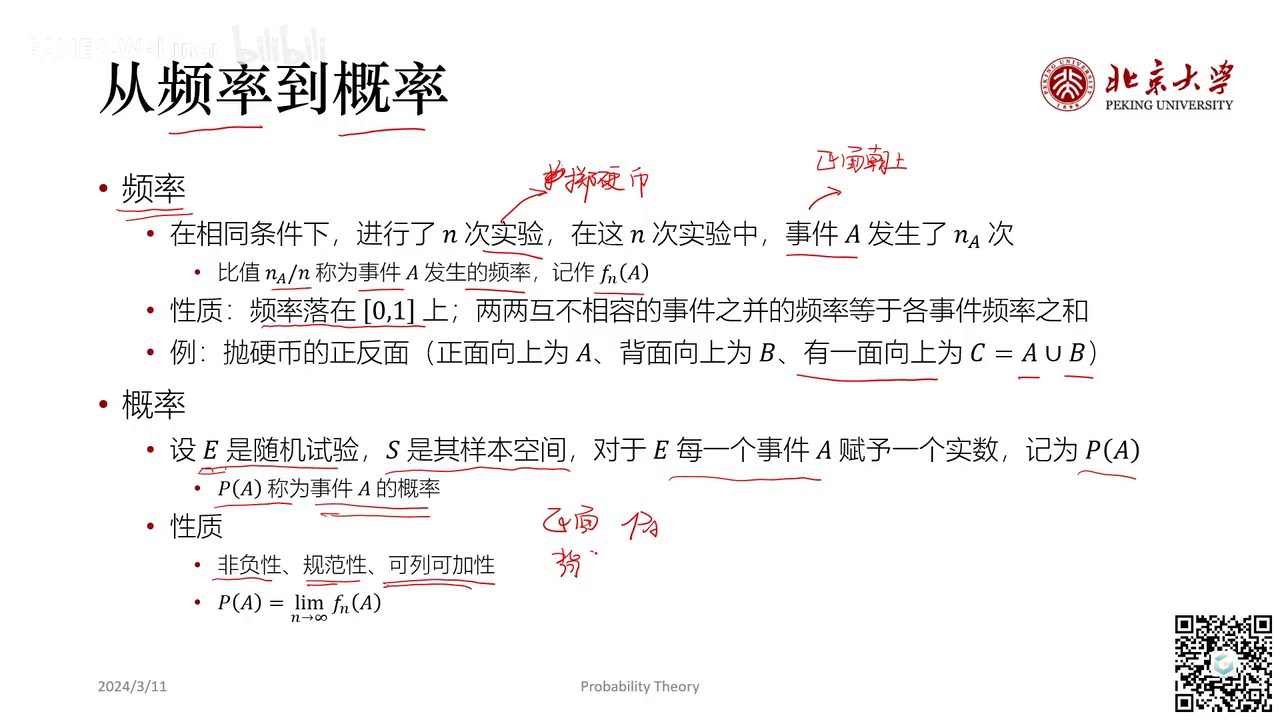
\includegraphics[width=0.92\textwidth]{figures/fig_01_freq.jpg}
\caption{从频率到概率：频率的定义、性质，以及概率的公理化定义\vtag}
\end{figure}
\srcnote{00:06:30--00:06:45}
\end{minipage}


频率有两条显然的性质：它落在 $[0,1]$ 上；两个互不相容的事件之并的频率等于各自频率之和。比如抛硬币时，正面向上记为 $A$，背面向上记为 $B$，“有一面向上”记为 $C=A\cup B$，则 $f_n(C)=f_n(A)+f_n(B)$。

\subsection{概率的公理化定义}

设 $E$ 是随机试验，$S$ 是它的样本空间。对 $E$ 的每一个事件 $A$ 赋予一个实数 $P(A)$，称为事件 $A$ 的概率。它需要满足三条性质：非负性，即概率不能是负的；规范性，即整个样本空间的概率为一，从而概率总落在零到一之间；可列可加性，即若干个两两互不相容的事件之并的概率等于各自概率之和，这与频率的可加性完全一样。

讲者强调，我们还要让这个定义与直觉相符：当试验次数趋于无穷时，频率 $f_n(A)$ 会趋向于 $P(A)$，
\begin{equation}
P(A)=\lim_{n\to\infty} f_n(A).
\end{equation}
只有这样定义的 $P$ 才能反映我们所理解的“概率”的含义。这一点后面会由大数定律严格说明。

\begin{knowledgebox}{频率与概率的区别}
频率是做完试验之后算出来的数，每做一组试验都可能不同；概率是事件本身的属性，在做试验之前就已经确定。两者的桥梁是“试验次数趋于无穷”：频率在某种意义下收敛到概率。讲义作者补充：这里的收敛是“依概率收敛”，不是数列意义下的普通收敛，后文大数定律一节会解释二者的差别。
\end{knowledgebox}

\section{古典概型}

\subsection{定义}

最简单的概率模型是古典概型，也叫等可能概型。它有两个条件：试验的样本空间只包含有限个元素；试验中每个基本事件发生的可能性相同。抛硬币、掷骰子都是典型例子。抛硬币时只有正面向上和背面向上两种结果，讲者开玩笑说也许有人会“杠”能不能侧边立住，这里不考虑这种情况，认为它不可能发生。

\noindent\begin{minipage}{\textwidth}
\begin{figure}[H]
\centering
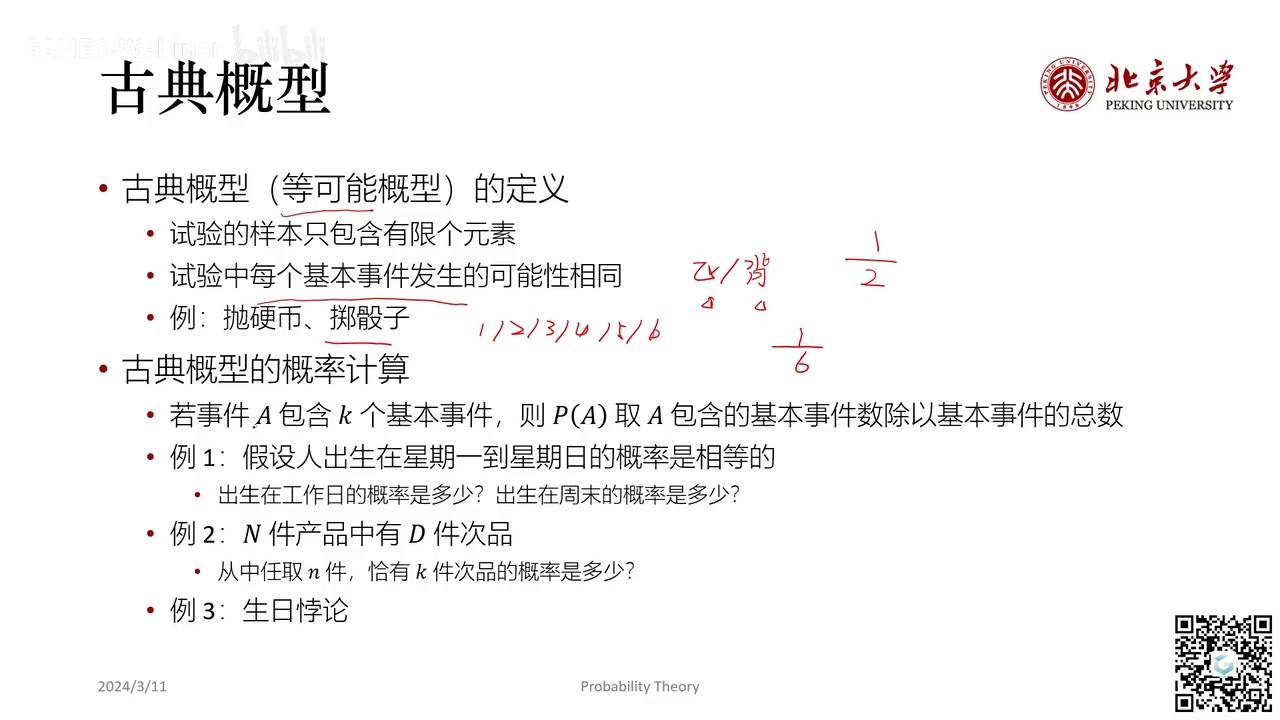
\includegraphics[width=0.92\textwidth]{figures/fig_02_classical.jpg}
\caption{古典概型的定义与三个例子\vtag}
\end{figure}
\srcnote{00:09:00--00:09:15}
\end{minipage}


在古典概型中，若事件 $A$ 包含 $k$ 个基本事件，样本空间共有 $n$ 个基本事件，则
\begin{equation}
P(A)=\frac{k}{n}.
\end{equation}

\subsection{三个例子}

\textbf{例一：出生在星期几。}假设一个人出生在星期一到星期日的概率相等。一周有七天，其中工作日五天，所以出生在工作日的概率是 $5/7$，出生在周末的概率是 $2/7$。

\textbf{例二：抽次品。}$N$ 件产品中有 $D$ 件次品，从中任取 $n$ 件，恰有 $k$ 件次品的概率是多少？讲者的思路是数基本事件：在 $D$ 件次品中选 $k$ 件，在 $N-D$ 件正品中选 $n-k$ 件，再除以从 $N$ 件中选 $n$ 件的总数：
\begin{equation}
P=\frac{\binom{D}{k}\binom{N-D}{n-k}}{\binom{N}{n}}.
\end{equation}

\noindent\begin{minipage}{\textwidth}
\begin{figure}[H]
\centering
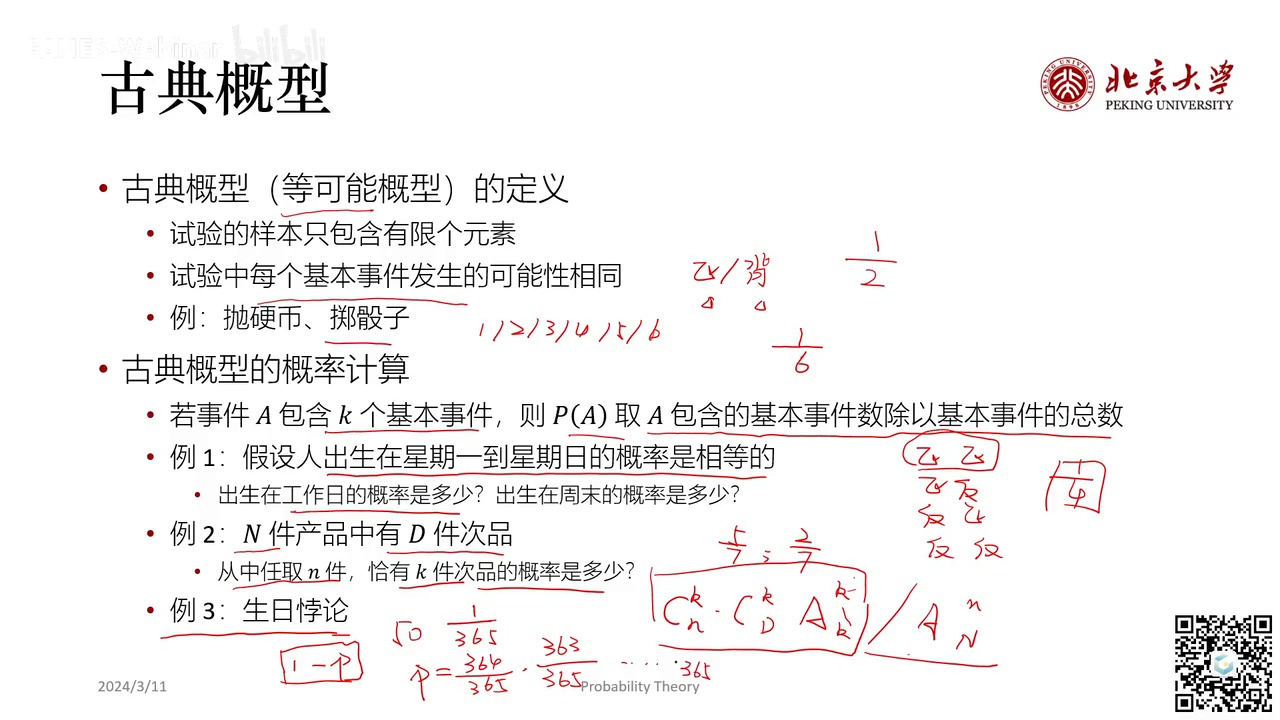
\includegraphics[width=0.92\textwidth]{figures/fig_03_classical_note.jpg}
\caption{讲者在古典概型例题旁的板书\vtag}
\end{figure}
\srcnote{00:13:00--00:13:15}
\end{minipage}


\textbf{例三：生日悖论。}班上有 $50$ 名同学，至少有两人生日相同的概率是多少？按古典概型，每个人生在每一天的概率都认为相等，并忽略闰年，即每天 $1/365$。先算 50 人生日两两不同的概率：第一个人随便，第二个人要避开 1 天，……，第 50 个人要避开 49 天，
\begin{equation}
\bar p=\frac{365\times 364\times\cdots\times 316}{365^{50}}.
\end{equation}
最后一个因子是 $365-49=316$。这个概率相当低，所以“至少两人同生日”的概率很高。讲者提醒大家回想：从小到大的班上基本都会有两个同学生日在同一天，原因就在这里。

\begin{warningbox}{生日问题的具体数值}
讲者口头估计“不存在两人同生日”的概率在百分之一左右的量级。讲义作者按上式核算，其精确值约为 $0.0296$，即约 $3\%$，所以至少两人同生日的概率约为 $97\%$。数量级的结论（非常接近必然）不变，但具体数值以此为准。
\end{warningbox}

\section{条件概率与贝叶斯公式}

\subsection{条件概率与乘法定理}

古典概型只会“数数”，还不够用，还需要一个对概率非常重要的概念：条件概率。事件 $A$ 发生的条件下事件 $B$ 发生的概率记作 $P(B\mid A)$，定义为
\begin{equation}
P(B\mid A)=\frac{P(AB)}{P(A)},
\end{equation}
即 $A$ 与 $B$ 同时发生的概率除以 $A$ 发生的概率。把它移项，就得到乘法定理 $P(AB)=P(B\mid A)P(A)$。

\noindent\begin{minipage}{\textwidth}
\begin{figure}[H]
\centering
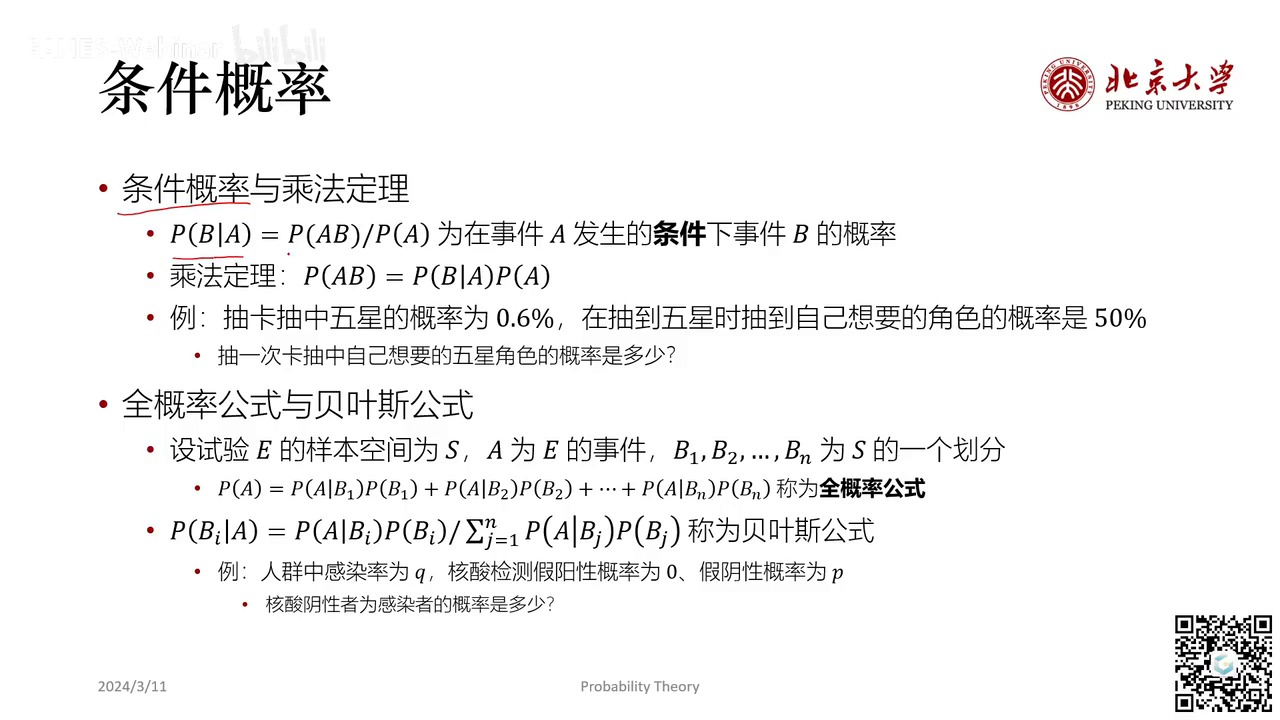
\includegraphics[width=0.92\textwidth]{figures/fig_04_conditional.jpg}
\caption{条件概率、乘法定理、全概率公式与贝叶斯公式\vtag}
\end{figure}
\srcnote{00:14:00--00:14:15}
\end{minipage}


讲者举了一个抽卡的例子：抽一次卡抽中五星的概率是 $0.6\%$，在抽到五星时抽到自己想要的角色的概率是 $50\%$。那么抽一次卡抽中自己想要的五星角色的概率是多少？首先要抽中五星，在抽中五星的情况下再抽到想要的角色，由乘法定理，
\begin{equation}
0.6\%\times 50\%=0.3\%.
\end{equation}

\subsection{全概率公式}

设试验 $E$ 的样本空间为 $S$，$B_1,B_2,\dots,B_n$ 为 $S$ 的一个划分。所谓划分，是说它们两两之间不可能同时发生，并且合在一起覆盖了所有可能性，比如掷骰子时“掷出一点”到“掷出六点”就是样本空间的一个划分。此时
\begin{equation}
P(A)=P(A\mid B_1)P(B_1)+P(A\mid B_2)P(B_2)+\cdots+P(A\mid B_n)P(B_n).
\end{equation}
直观地说：在每一种情况 $B_i$ 下考察事件 $A$ 发生的概率，按各情况的概率加权求和，就得到 $A$ 发生的总概率。这称为全概率公式。

\subsection{贝叶斯公式}

反过来，已知 $A$ 发生了，想问它“来自”哪一种情况 $B_i$ 的概率。利用乘法定理，$A$ 与 $B_i$ 同时发生的概率等于 $B_i$ 发生的概率乘以 $B_i$ 发生时 $A$ 也发生的概率；分母用全概率公式展开，得到贝叶斯公式
\begin{equation}
P(B_i\mid A)=\frac{P(A\mid B_i)P(B_i)}{\sum_{j=1}^{n}P(A\mid B_j)P(B_j)}.
\end{equation}

\noindent\begin{minipage}{\textwidth}
\begin{figure}[H]
\centering
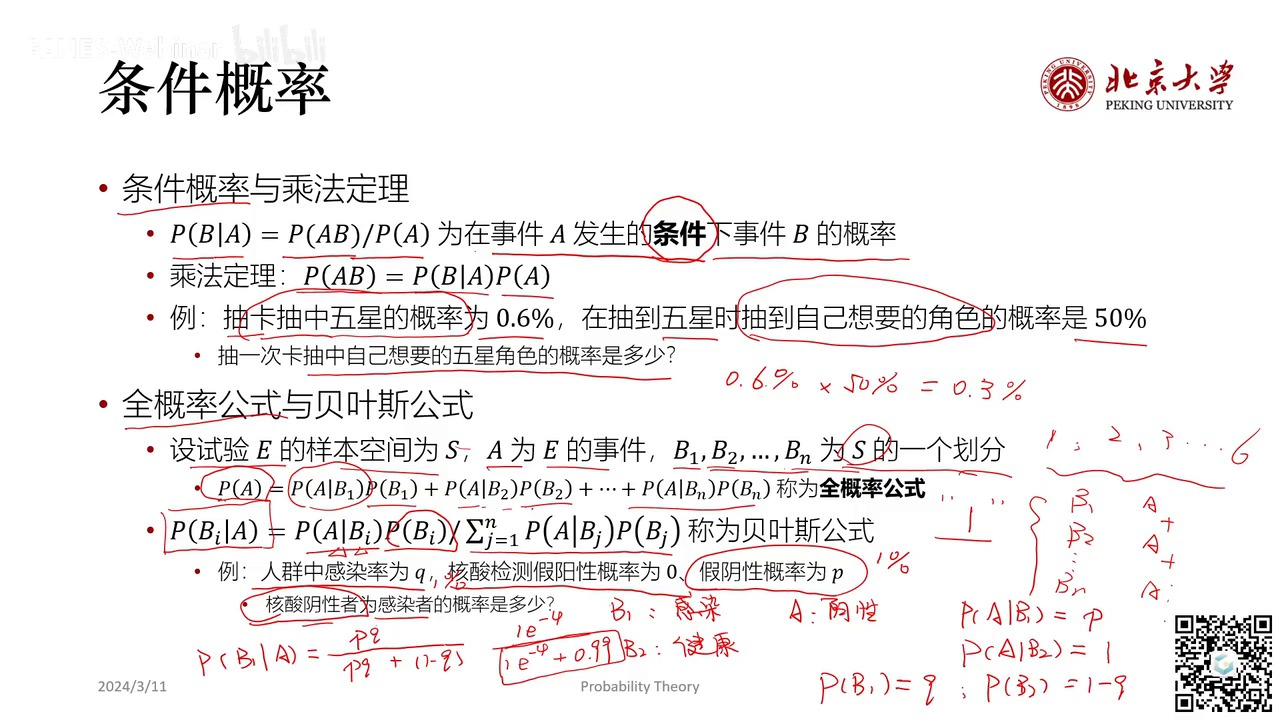
\includegraphics[width=0.92\textwidth]{figures/fig_05_bayes_note.jpg}
\caption{讲者在课件上用核酸检测的例子演算贝叶斯公式\vtag}
\end{figure}
\srcnote{00:23:30--00:23:45}
\end{minipage}


讲者的例子是核酸检测：人群中感染者的比例为 $q$；假阳性概率为 $0$，即没感染的人一定被检测为阴性；假阴性概率为 $p$，即感染者有 $p$ 的概率被检测为阴性。问：核酸阴性的人是感染者的概率是多少？套用贝叶斯公式，记“感染”为 $B$，“检测阴性”为 $A$：
\begin{equation}
P(B\mid A)=\frac{p\,q}{p\,q+1\cdot(1-q)}.
\end{equation}

\begin{practicebox}{读懂这个式子}
讲者带大家检查了几个极端情形，读者可以自己验证：
\begin{enumerate}
\item 若检测完美无瑕，假阴性概率 $p=0$，则阴性者是感染者的概率为 $0$。
\item 若人群中感染者比例 $q$ 很低，这个概率也很低，这与直觉相符。
\item 若人群中所有人都是感染者，即 $q=1$，则上式等于 $1$：阴性者也一定是感染者。
\end{enumerate}
\end{practicebox}

\begin{knowledgebox}{贝叶斯公式的读法}
讲义作者补充一种常见读法：$P(B_i)$ 称为先验，是看到证据之前对各种情况的信念；$P(A\mid B_i)$ 称为似然，表示在某种情况下出现这个证据的可能性；$P(B_i\mid A)$ 称为后验，是看到证据后更新过的信念。分母只是归一化常数。图形学中重要性采样、去噪等方法里经常出现这种“先验乘似然”的结构。
\end{knowledgebox}

\section{随机变量与常见分布}

\subsection{随机变量的定义}

\noindent\begin{minipage}{\textwidth}
\begin{figure}[H]
\centering
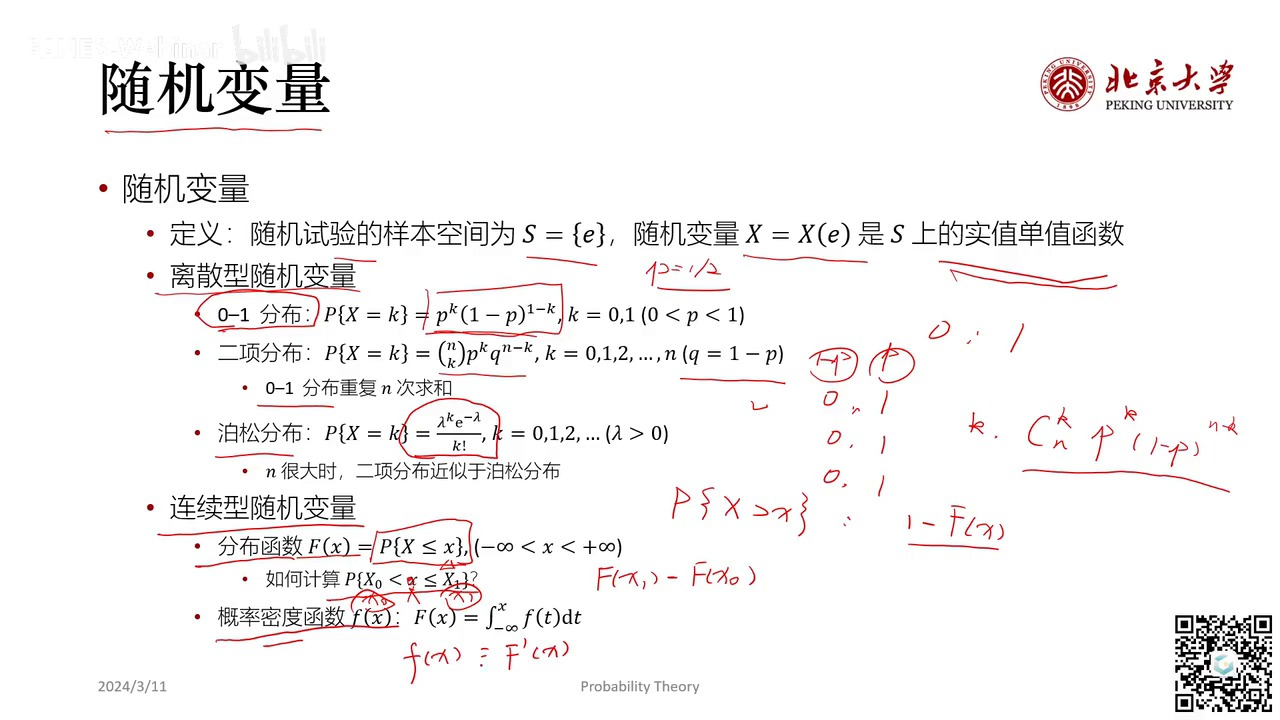
\includegraphics[width=0.92\textwidth]{figures/fig_06_rv.jpg}
\caption{随机变量的定义，离散型的三种分布和连续型的分布函数\vtag}
\end{figure}
\srcnote{00:30:45--00:31:00}
\end{minipage}


离开古典概型，就需要随机变量。设随机试验的样本空间为 $S=\{e\}$，随机变量 $X=X(e)$ 是定义在 $S$ 上的实值单值函数。它把每一个试验结果映射成一个实数，这样就能用分析的工具来研究随机现象。

\subsection{离散型随机变量}

\textbf{0--1 分布。}讲者举的例子是赌博：硬币可能经过精心设置，正反面的概率不同。设得一分的概率为 $p$，得零分的概率为 $1-p$，则得分为 $k$ 的概率为
\begin{equation}
P\{X=k\}=p^{k}(1-p)^{1-k},\qquad k=0,1\ (0<p<1).
\end{equation}

\textbf{二项分布。}把 0--1 分布独立重复 $n$ 次，统计成功次数：
\begin{equation}
P\{X=k\}=\binom{n}{k}p^{k}q^{n-k},\qquad k=0,1,\dots,n,\quad q=1-p.
\end{equation}
它很好理解：比如投 $n$ 次，要在其中选出 $k$ 次成功，成功的这 $k$ 次每次概率 $p$，失败的 $n-k$ 次每次概率 $1-p$，相乘再乘上选法数即可。

\textbf{泊松分布。}泊松分布是二项分布的极限情况：当 $n$ 很大、单次概率很小时，二项分布近似于泊松分布
\begin{equation}
P\{X=k\}=\frac{\lambda^{k}e^{-\lambda}}{k!},\qquad k=0,1,2,\dots\ (\lambda>0).
\end{equation}

\noindent\begin{minipage}{\textwidth}
\begin{figure}[H]
\centering
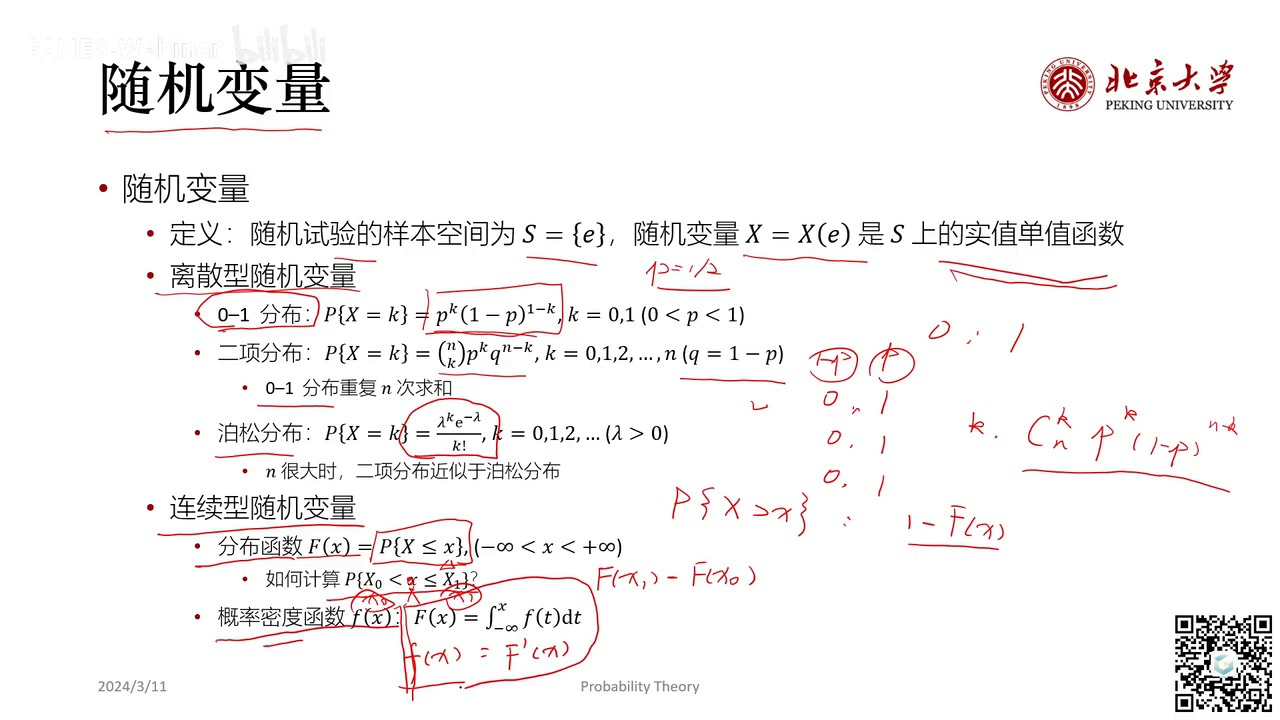
\includegraphics[width=0.92\textwidth]{figures/fig_07_rv_note.jpg}
\caption{讲者在离散分布旁的批注\vtag}
\end{figure}
\srcnote{00:31:00--00:31:15}
\end{minipage}


\subsection{连续型随机变量与分布函数}

有离散型，就有连续型：得到的随机变量的值不一定是离散的，可以取一个区间上的任意实数。为了统一描述两者，引入分布函数
\begin{equation}
F(x)=P\{X\le x\},\qquad -\infty<x<+\infty.
\end{equation}
有人会问为什么不定义成“大于等于”，讲者说这只是一种惯例。有了分布函数，计算 $X$ 落在区间上的概率就很方便：$P\{x_1<X\le x_2\}=F(x_2)-F(x_1)$。若要算 $X$ 大于某个值的概率，就是 $1-F(x)$，因为随机变量总是有值的，它落在 $(-\infty,+\infty)$ 内的概率为一。

对于连续型随机变量，还有一个非常重要的函数，叫概率密度函数 $f(x)$。它与分布函数是导函数与原函数的关系：
\begin{equation}
F(x)=\int_{-\infty}^{x} f(t)\,\mathrm{d}t .
\end{equation}

\subsection{三种常见的连续分布}

\noindent\begin{minipage}{\textwidth}
\begin{figure}[H]
\centering
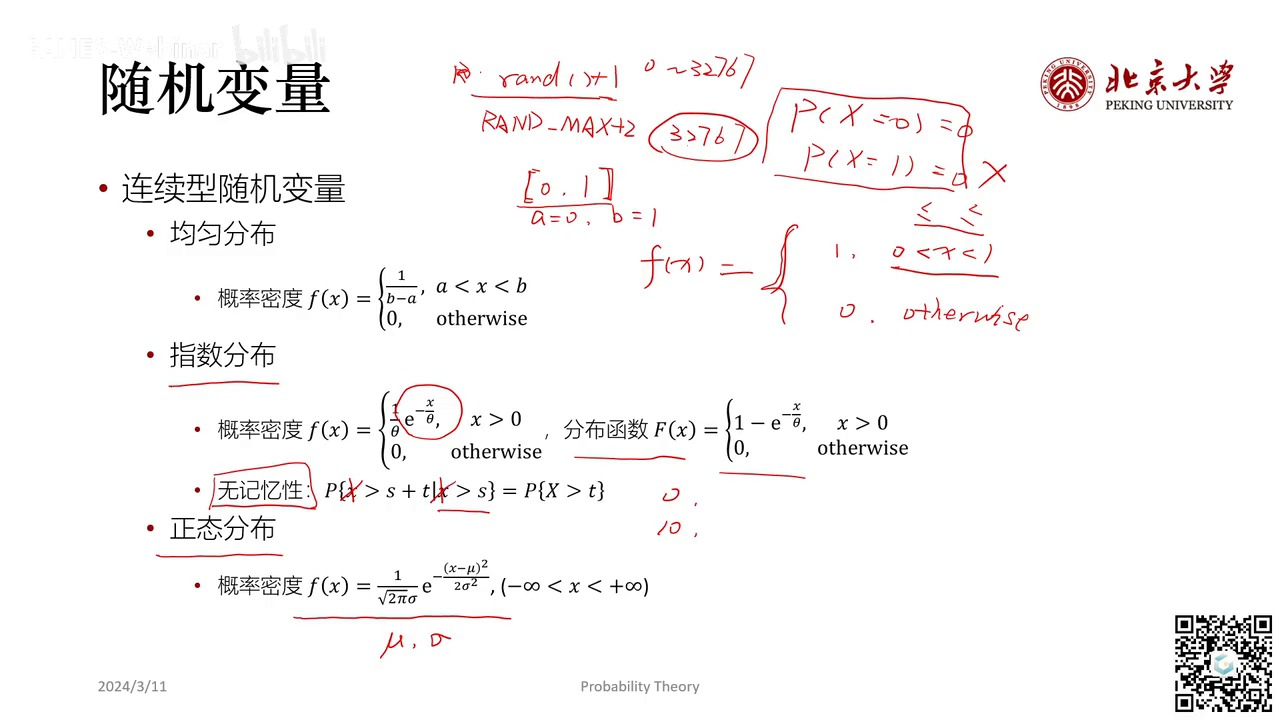
\includegraphics[width=0.92\textwidth]{figures/fig_08_continuous.jpg}
\caption{连续型随机变量：均匀分布、指数分布与正态分布\vtag}
\end{figure}
\srcnote{00:36:15--00:36:30}
\end{minipage}


\textbf{均匀分布。}在区间 $(a,b)$ 上均匀分布的概率密度为：在区间内取 $1/(b-a)$，否则为 $0$。有同学会问区间端点用大于号还是大于等于号，讲者指出，在概率的意义上，对连续型随机变量来说单个点的概率为零，所以端点取不取并不影响。

\begin{warningbox}{程序里的“均匀分布”并不连续}
讲者以 C 语言为例：用 \texttt{rand()/RAND\_MAX} 生成 $[0,1]$ 上的随机数。在 Windows 平台上 \texttt{RAND\_MAX} 是 $32767$，\texttt{rand()} 的结果是 $0$ 到 $32767$ 的整数，所以得到的数两个端点都可取，并且它只有三万多种可能取值，取到某个确切值的概率并不是零。如果不想包含端点，可以把分子加一、分母加二，即 \texttt{(rand()+1)/(RAND\_MAX+2)}，这样左右端点都取不到。写蒙特卡洛程序时要留意随机数生成器的这些细节。
\end{warningbox}

\textbf{指数分布。}概率密度和分布函数分别为
\begin{equation}
f(x)=\begin{cases}\dfrac{1}{\theta}e^{-x/\theta}, & x>0,\\[4pt] 0, & \text{otherwise},\end{cases}
\qquad
F(x)=\begin{cases}1-e^{-x/\theta}, & x>0,\\ 0, & \text{otherwise}.\end{cases}
\end{equation}
它最重要的特点是无记忆性：
\begin{equation}
P\{X>s+t\mid X>s\}=P\{X>t\}.
\end{equation}
讲者的通俗解释是：你之前发生了什么我不知道，无论你现在已经得了零分还是十分，你想再获得二十分的概率都相同。

\textbf{正态分布。}概率密度为
\begin{equation}
f(x)=\frac{1}{\sqrt{2\pi}\,\sigma}\,e^{-\frac{(x-\mu)^2}{2\sigma^2}},\qquad -\infty<x<+\infty,
\end{equation}
其中 $\mu$ 和 $\sigma$ 都是常量参数。它看起来复杂，但它是最重要的分布，本讲最后的中心极限定理会说明原因。

\section{数学期望与方差}

\subsection{数学期望}

\noindent\begin{minipage}{\textwidth}
\begin{figure}[H]
\centering
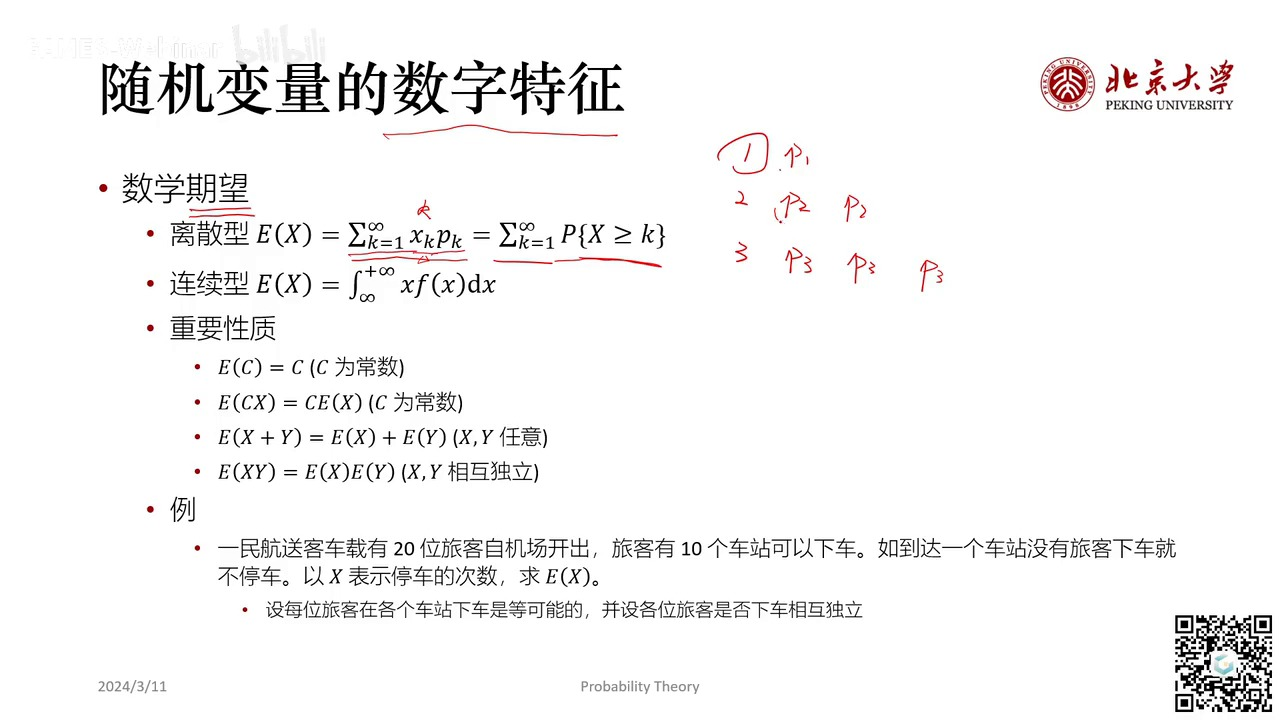
\includegraphics[width=0.92\textwidth]{figures/fig_09_expectation.jpg}
\caption{数学期望的定义、重要性质与停车次数的例子\vtag}
\end{figure}
\srcnote{00:38:00--00:38:15}
\end{minipage}


离散型随机变量的数学期望为 $E(X)=\sum_{k=1}^{\infty}x_k p_k$，连续型为 $E(X)=\int_{-\infty}^{+\infty}x f(x)\,\mathrm{d}x$。对于取正整数值的离散型随机变量，还有一个等价形式
\begin{equation}
E(X)=\sum_{k=1}^{\infty}k\,P\{X=k\}=\sum_{k=1}^{\infty}P\{X\ge k\}.
\end{equation}
讲者的解释是“分层累加”：以 $P\{X\ge 1\}$ 的概率获得从零到一的那一份，以 $P\{X\ge 2\}$ 的概率再获得从一到二的那一份，以此类推，把各层加起来就是期望。

\noindent\begin{minipage}{\textwidth}
\begin{figure}[H]
\centering
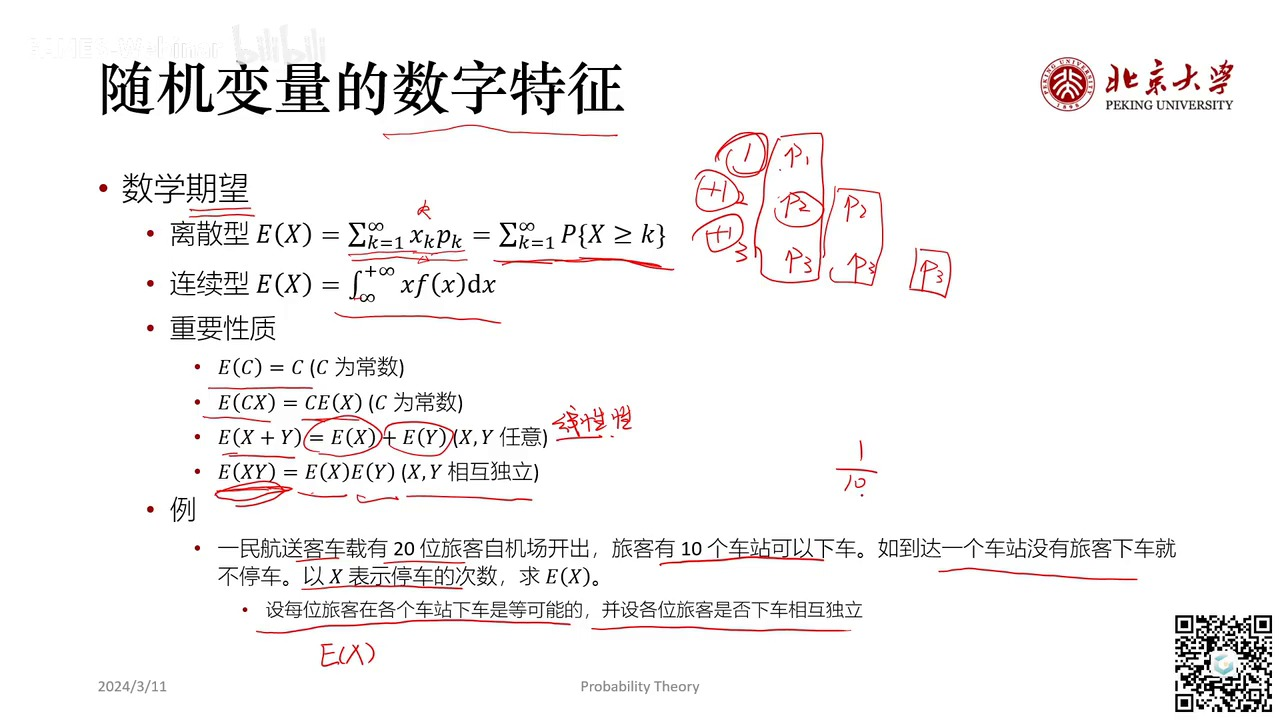
\includegraphics[width=0.92\textwidth]{figures/fig_10_expectation_note.jpg}
\caption{讲者对期望第二种写法的板书推导\vtag}
\end{figure}
\srcnote{00:41:00--00:41:15}
\end{minipage}


期望有四条重要性质：$E(C)=C$；$E(CX)=CE(X)$；对任意两个随机变量 $E(X+Y)=E(X)+E(Y)$；若 $X,Y$ 相互独立，则 $E(XY)=E(X)E(Y)$。讲者特别指出，第三条对任意随机变量都成立，不要求独立；第四条才需要独立。

\begin{practicebox}{停车次数的期望}
课件例题：一民航送客车载有 $20$ 位旅客自机场开出，旅客有 $10$ 个车站可以下车，到达一个车站若没有旅客下车就不停车。以 $X$ 表示停车次数，求 $E(X)$。设每位旅客在各车站下车是等可能的，且各旅客是否下车相互独立。

思路：对第 $i$ 个车站引入指示变量 $X_i$，有人下车取一，否则取零，则 $X=X_1+\cdots+X_{10}$。每位旅客在某站下车的概率为十分之一，不在该站下车的概率为 $0.9$，所以某站没有人下车的概率为 $0.9^{20}$，从而 $E(X_i)=1-0.9^{20}$。由期望的可加性（不需要独立），
\begin{equation}
E(X)=10\left(1-0.9^{20}\right)\approx 8.784 .
\end{equation}
数值由讲义作者补算。
\end{practicebox}

\subsection{方差}

有了期望，就可以定义方差。方差度量随机变量与其均值（即期望）之间的偏离程度：
\begin{equation}
D(X)=\operatorname{Var}(X)=E\{[X-E(X)]^2\},
\end{equation}
$\sigma(X)=\sqrt{D(X)}$ 称为标准差或均方差。讲者解释“均值”这个名字的来历：大量重复试验所得的平均会趋向于数学期望，所以数学期望又称为均值。

\noindent\begin{minipage}{\textwidth}
\begin{figure}[H]
\centering
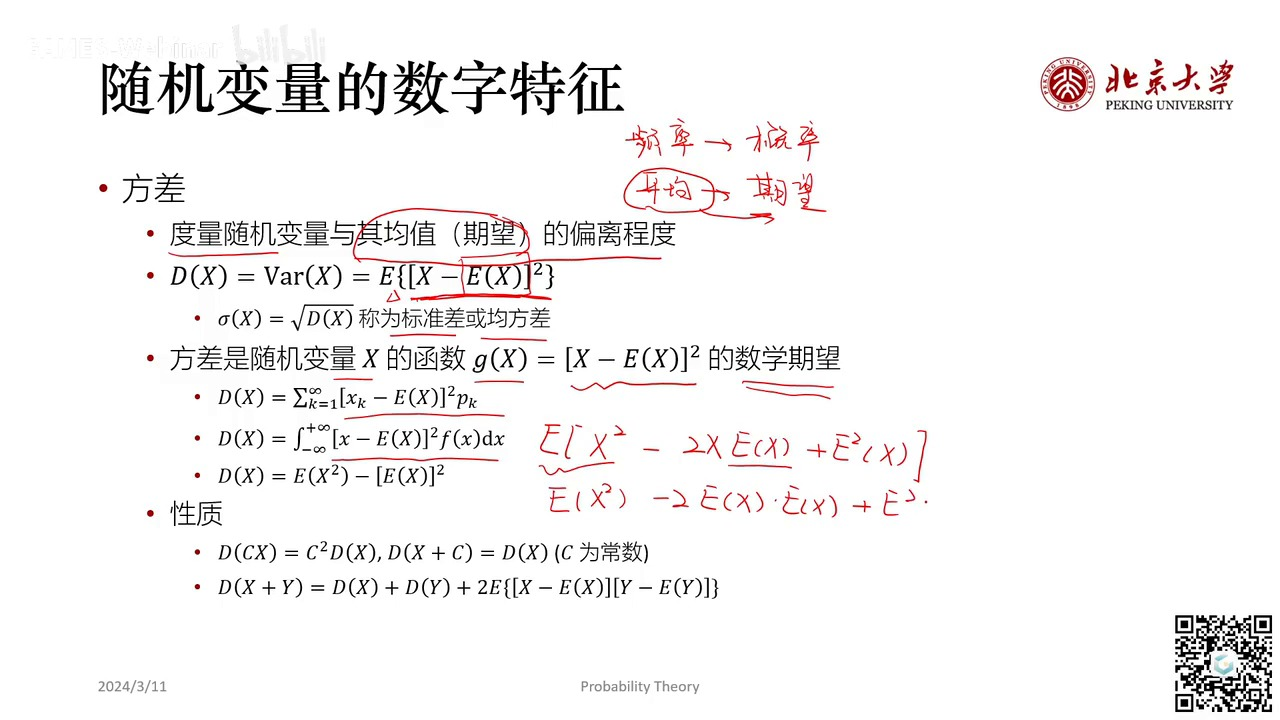
\includegraphics[width=0.92\textwidth]{figures/fig_11_variance.jpg}
\caption{方差的定义、计算公式与性质\vtag}
\end{figure}
\srcnote{00:44:45--00:45:00}
\end{minipage}


方差是随机变量的函数 $g(X)=[X-E(X)]^2$ 的数学期望。离散情形为 $\sum_k[x_k-E(X)]^2p_k$，连续情形为 $\int[x-E(X)]^2f(x)\,\mathrm{d}x$。把平方展开，利用期望的线性，可以得到最常用的计算公式
\begin{equation}
D(X)=E(X^2)-[E(X)]^2 .
\end{equation}
方差的性质：$D(CX)=C^2D(X)$，$D(X+C)=D(X)$；以及
\begin{equation}
D(X+Y)=D(X)+D(Y)+2E\{[X-E(X)][Y-E(Y)]\}.
\end{equation}
最后一项正是下文的协方差；当 $X,Y$ 独立时它为零，方差才可以直接相加。

\begin{warningbox}{期望可加，方差不一定可加}
期望的可加性对任意随机变量成立，但方差的可加性需要两者不相关（独立是充分条件）。另外，常数倍进入方差时要平方：$D(CX)=C^2D(X)$，而不是 $CD(X)$。这两点在估计蒙特卡洛积分误差时经常用到。
\end{warningbox}

\section{两个分布的推导}

讲者回过头来，用刚有的期望和方差两个工具，推导前面提到的两个分布。

\subsection{泊松分布}

\noindent\begin{minipage}{\textwidth}
\begin{figure}[H]
\centering
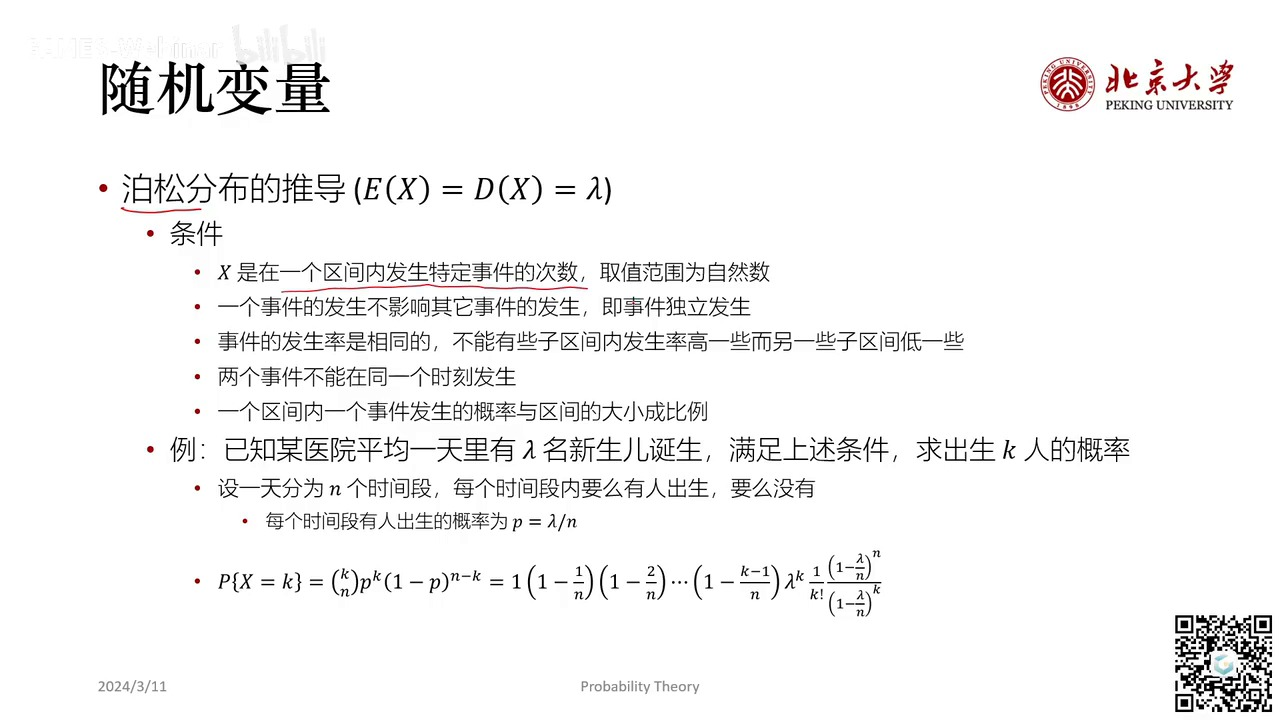
\includegraphics[width=0.92\textwidth]{figures/fig_12_poisson.jpg}
\caption{泊松分布的推导：条件与新生儿的例子\vtag}
\end{figure}
\srcnote{00:46:15--00:46:30}
\end{minipage}


泊松分布满足 $E(X)=D(X)=\lambda$。$X$ 表示一个区间内发生特定事件的次数，取值为自然数。它要求五个条件：一个事件的发生不影响其他事件的发生，即事件独立发生；事件的发生率相同，不能某些子区间发生率高而另一些低；两个事件不能在同一个时刻发生；一个区间内一个事件发生的概率与区间大小成正比。

例子：已知某医院平均一天有 $\lambda$ 名新生儿诞生，且满足上述条件，求一天出生 $k$ 人的概率。把一天分为 $n$ 个时间段，每个时间段内要么有人出生，要么没有。由于二项分布的期望是 $np$，要让它等于 $\lambda$，每个时间段有人出生的概率就得是 $p=\lambda/n$。一天有 $k$ 人出生的概率是典型的二项分布：
\begin{equation}
P\{X=k\}=\binom{n}{k}p^{k}(1-p)^{n-k}
=1\left(1-\frac{1}{n}\right)\cdots\left(1-\frac{k-1}{n}\right)\frac{\lambda^{k}}{k!}\,
\frac{\left(1-\frac{\lambda}{n}\right)^{n}}{\left(1-\frac{\lambda}{n}\right)^{k}} .
\end{equation}

\noindent\begin{minipage}{\textwidth}
\begin{figure}[H]
\centering
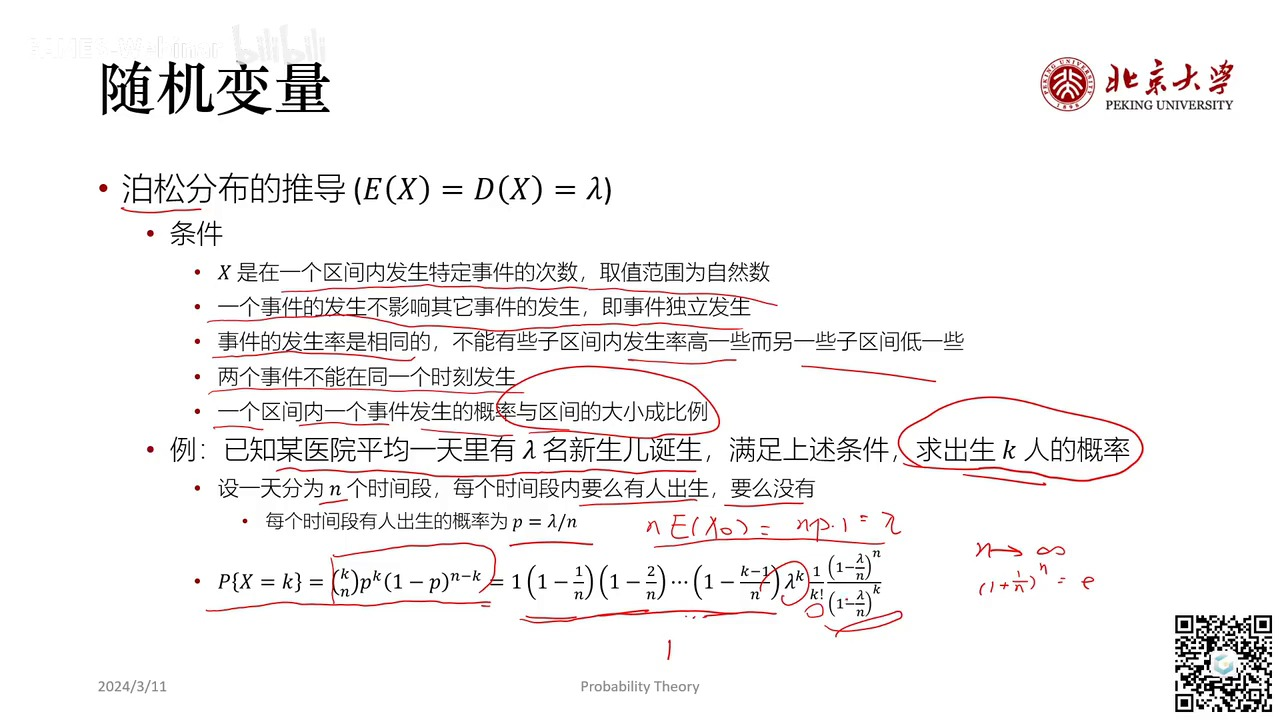
\includegraphics[width=0.92\textwidth]{figures/fig_13_poisson_limit.jpg}
\caption{讲者对 $n\to\infty$ 时各因子极限的批注\vtag}
\end{figure}
\srcnote{00:49:30--00:49:45}
\end{minipage}


令 $n\to\infty$：前面那些形如 $1-j/n$ 的因子都趋于一，分母 $(1-\lambda/n)^k$ 也趋于一；而 $(1-\lambda/n)^n$ 趋于 $e^{-\lambda}$，这是高等数学里很熟悉的极限。于是得到泊松分布 $\lambda^k e^{-\lambda}/k!$。

\subsection{指数分布}

\noindent\begin{minipage}{\textwidth}
\begin{figure}[H]
\centering
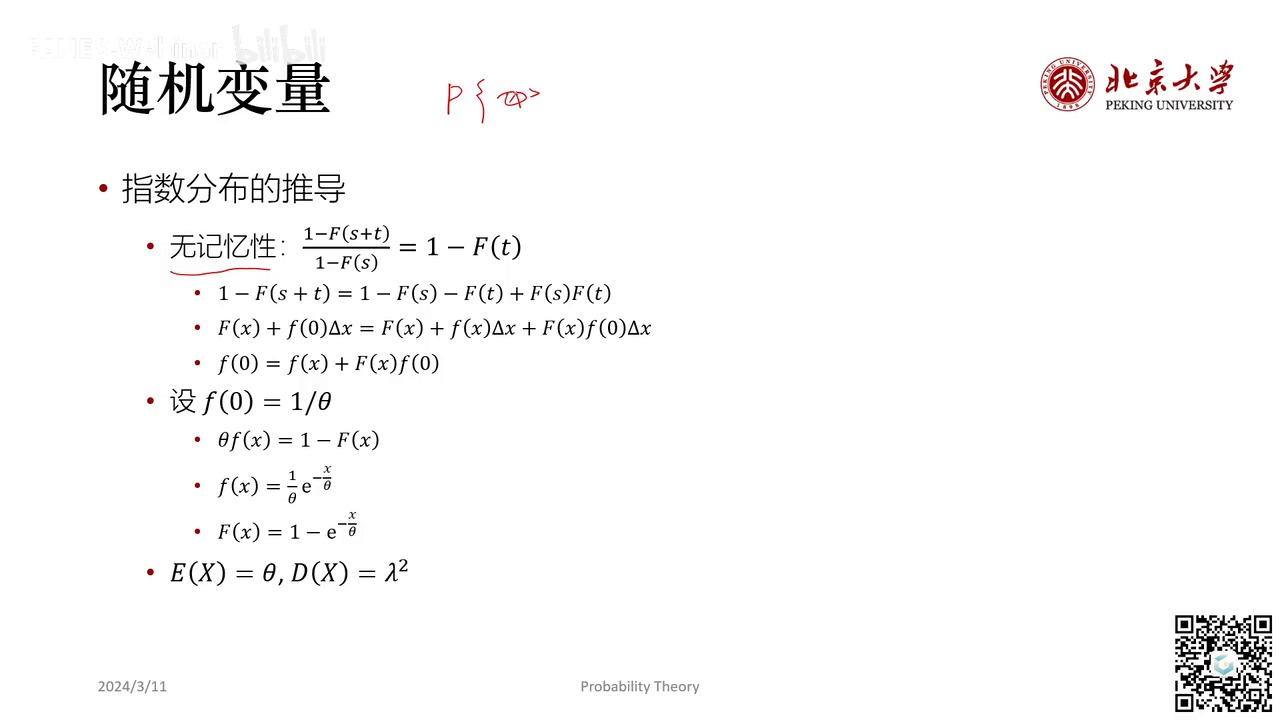
\includegraphics[width=0.92\textwidth]{figures/fig_14_exponential.jpg}
\caption{指数分布的推导：从无记忆性出发\vtag}
\end{figure}
\srcnote{00:50:15--00:50:30}
\end{minipage}


讲者说指数分布最重要的特点是无记忆性。把无记忆性用分布函数写出来：
\begin{equation}
\frac{1-F(s+t)}{1-F(s)}=1-F(t),
\end{equation}
即 $1-F(s+t)=1-F(s)-F(t)+F(s)F(t)$。这对任意正数 $s,t$ 都成立。取 $s=x$、$t=\Delta x$，并利用 $F(\Delta x)\approx F(0)+f(0)\Delta x$ 以及 $F(0)=0$，得到
\begin{equation}
F(x)+f(x)\Delta x=F(x)+f(0)\Delta x-F(x)f(0)\Delta x,
\end{equation}
从而 $f(x)=f(0)-f(0)F(x)$。

\noindent\begin{minipage}{\textwidth}
\begin{figure}[H]
\centering
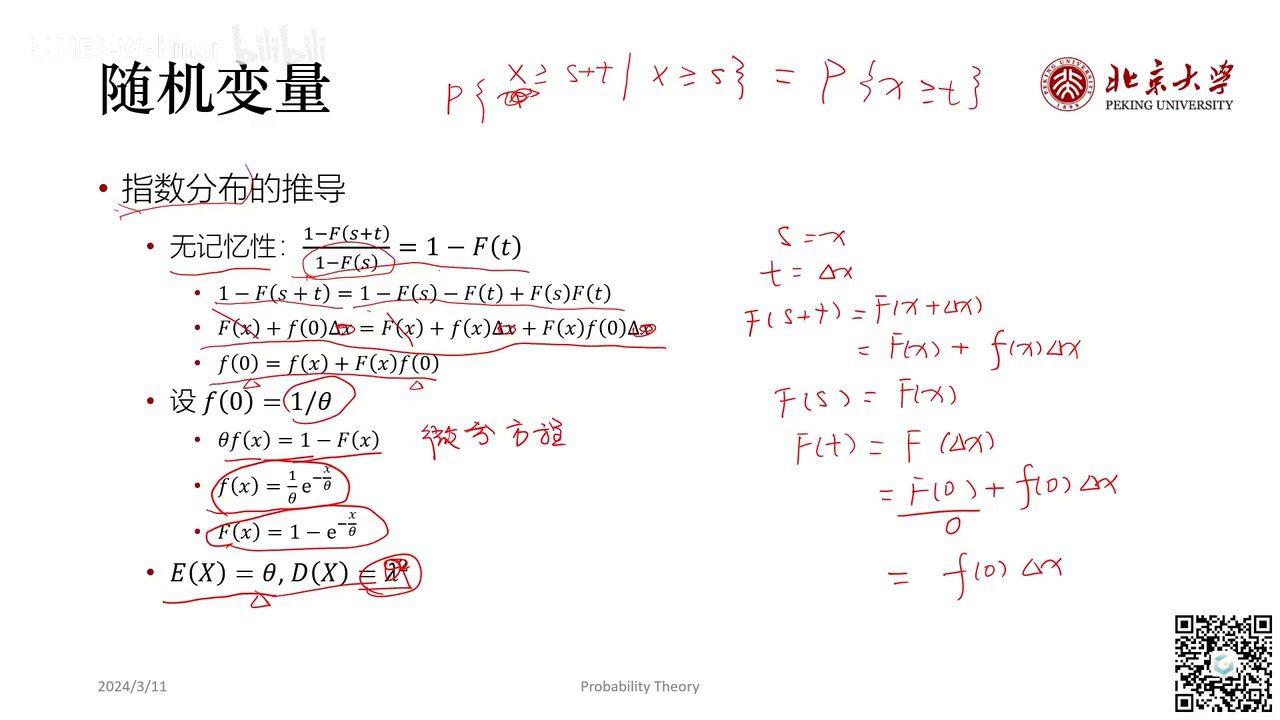
\includegraphics[width=0.92\textwidth]{figures/fig_15_exponential_note.jpg}
\caption{讲者在推导旁写出微分方程的求解过程\vtag}
\end{figure}
\srcnote{00:53:30--00:53:45}
\end{minipage}


设 $f(0)=1/\theta$，则 $\theta f(x)=1-F(x)$，这是关于 $F$ 的一阶线性微分方程，解得
\begin{equation}
f(x)=\frac{1}{\theta}e^{-x/\theta},\qquad F(x)=1-e^{-x/\theta},
\end{equation}
并且 $E(X)=\theta$，$D(X)=\theta^2$。

\begin{importantbox}{无记忆性与指数分布互相刻画}
讲者总结：无记忆性是指数分布的性质；反过来，从无记忆性出发也一定会导出指数分布。两者可以看作是等价的。在图形学中，光在均匀介质中“走多远才发生一次散射”的自由程就服从指数分布，正是因为介质没有“记忆”（这一应用由讲义作者补充）。
\end{importantbox}

\section{协方差与矩}

\subsection{协方差与相关系数}

\noindent\begin{minipage}{\textwidth}
\begin{figure}[H]
\centering
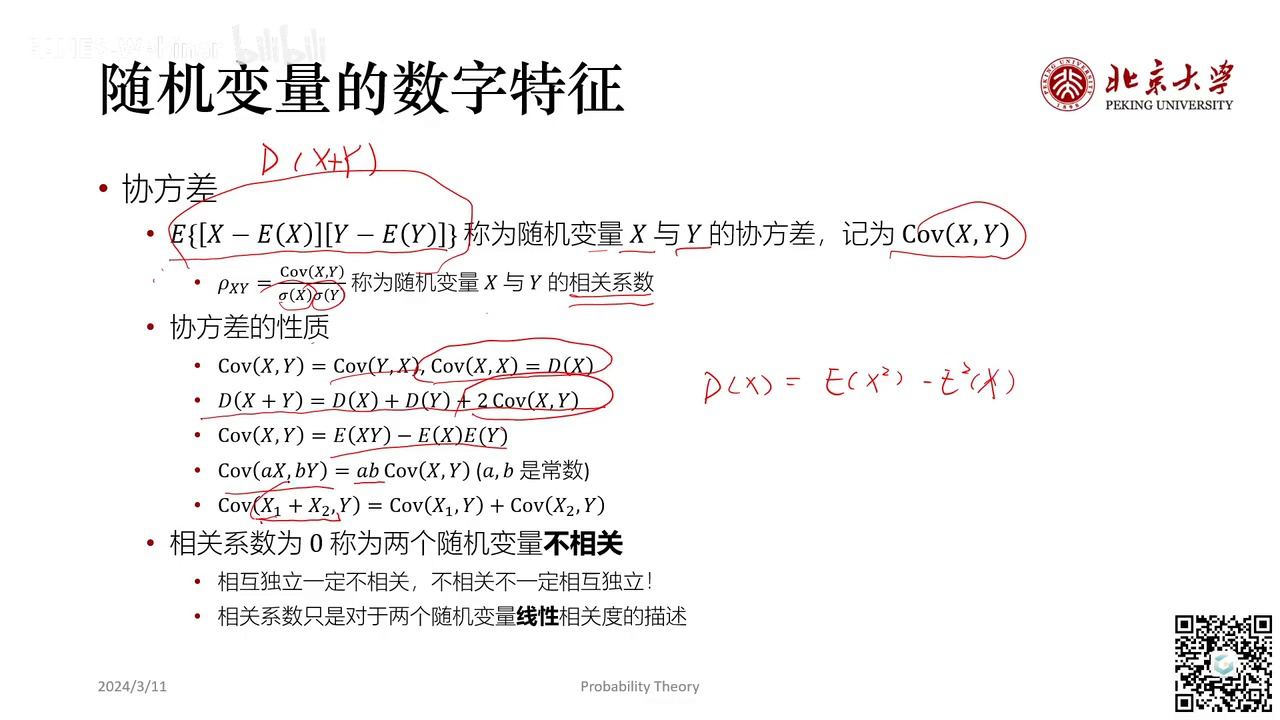
\includegraphics[width=0.92\textwidth]{figures/fig_16_covariance.jpg}
\caption{协方差的定义、性质与相关系数\vtag}
\end{figure}
\srcnote{00:55:45--00:56:00}
\end{minipage}


称 $E\{[X-E(X)][Y-E(Y)]\}$ 为随机变量 $X$ 与 $Y$ 的协方差，记为 $\operatorname{Cov}(X,Y)$。借助协方差可以定义相关系数
\begin{equation}
\rho_{XY}=\frac{\operatorname{Cov}(X,Y)}{\sigma(X)\sigma(Y)} .
\end{equation}
协方差有以下性质：$\operatorname{Cov}(X,Y)=\operatorname{Cov}(Y,X)$，$\operatorname{Cov}(X,X)=D(X)$；$D(X+Y)=D(X)+D(Y)+2\operatorname{Cov}(X,Y)$；$\operatorname{Cov}(X,Y)=E(XY)-E(X)E(Y)$；$\operatorname{Cov}(aX,bY)=ab\operatorname{Cov}(X,Y)$；$\operatorname{Cov}(X_1+X_2,Y)=\operatorname{Cov}(X_1,Y)+\operatorname{Cov}(X_2,Y)$。讲者说这些式子的证明很直接，把 $D(X)$ 按 $E(X^2)-[E(X)]^2$ 展开代入即可。

\noindent\begin{minipage}{\textwidth}
\begin{figure}[H]
\centering
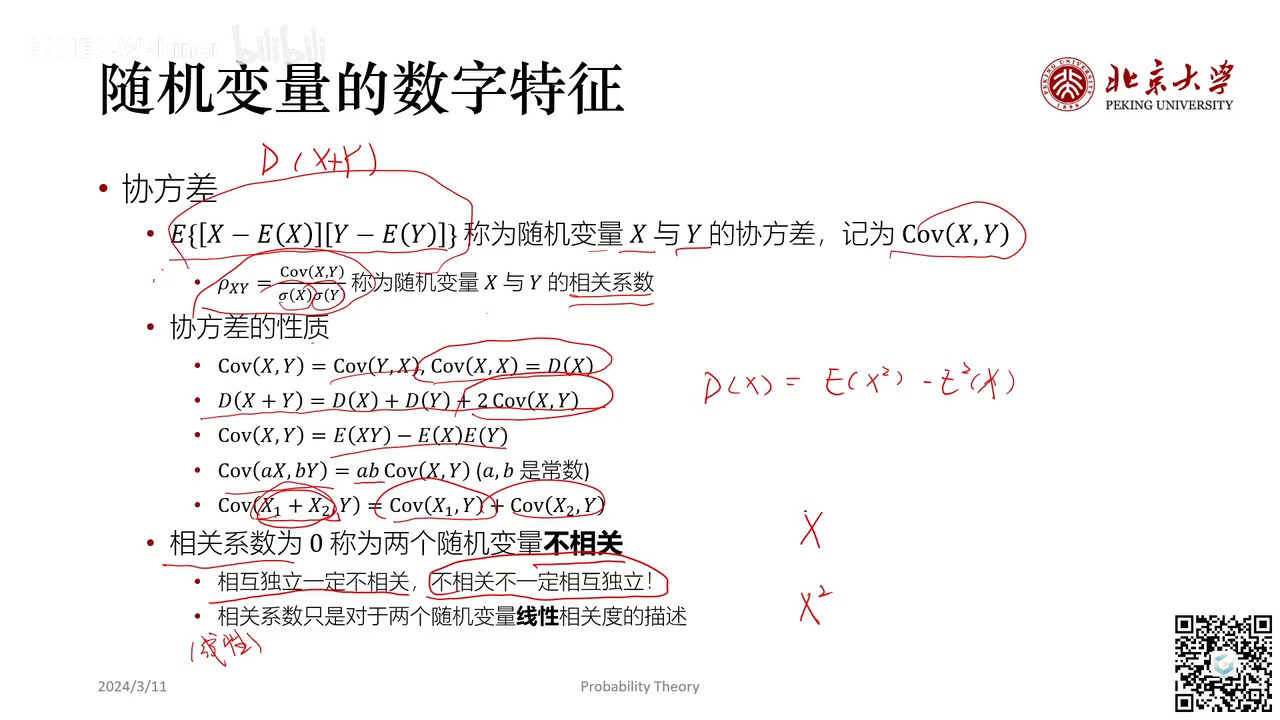
\includegraphics[width=0.92\textwidth]{figures/fig_17_covariance_note.jpg}
\caption{讲者用 $Y=X^2$ 的例子说明“不相关不等于独立”\vtag}
\end{figure}
\srcnote{00:57:00--00:57:15}
\end{minipage}


相关系数为零，称两个随机变量不相关。课件用加粗强调了两点：相互独立一定不相关，不相关不一定相互独立；相关系数只是对两个随机变量线性相关程度的描述。讲者的例子是：取 $Y=X^2$，这两个随机变量显然不是相互独立的，$X$ 取多少，$Y$ 就是它的平方；但如果去计算它们的相关系数，会发现它等于零。它们不是线性相关，而是平方相关。

\begin{warningbox}{不相关 $\neq$ 独立}
讲义作者补充让上例成立的条件：例如 $X$ 在 $[-1,1]$ 上均匀分布，则 $E(X)=0$，$E(XY)=E(X^3)=0$，所以 $\operatorname{Cov}(X,X^2)=0$。若 $X$ 的分布不关于零对称，协方差一般不为零。所以“相关系数为零”只能排除线性关系，不能用来判断独立。
\end{warningbox}

\subsection{矩}

\noindent\begin{minipage}{\textwidth}
\begin{figure}[H]
\centering

\includegraphics[width=0.92\textwidth]{figures/fig_18_moments.jpg}
\caption{矩的定义以及矩与期望、方差的关系\vtag}
\end{figure}
\srcnote{00:58:30--00:58:45}
\end{minipage}


矩是对随机变量性质的一种度量。设 $k=1,2,\dots$：
\begin{itemize}
\item $E(X^k)$ 称为 $X$ 的 $k$ 阶原点矩，简称 $k$ 阶矩；
\item $E\{[X-E(X)]^k\}$ 称为 $X$ 的 $k$ 阶中心矩；
\item $E(X^kY^l)$ 称为 $X$ 和 $Y$ 的 $k+l$ 阶混合矩；
\item $E\{[X-E(X)]^k[Y-E(Y)]^l\}$ 称为 $X$ 和 $Y$ 的 $k+l$ 阶混合中心矩。
\end{itemize}
于是数学期望是一阶原点矩，方差是二阶中心矩，协方差是二阶混合中心矩。

\noindent\begin{minipage}{\textwidth}
\begin{figure}[H]
\centering
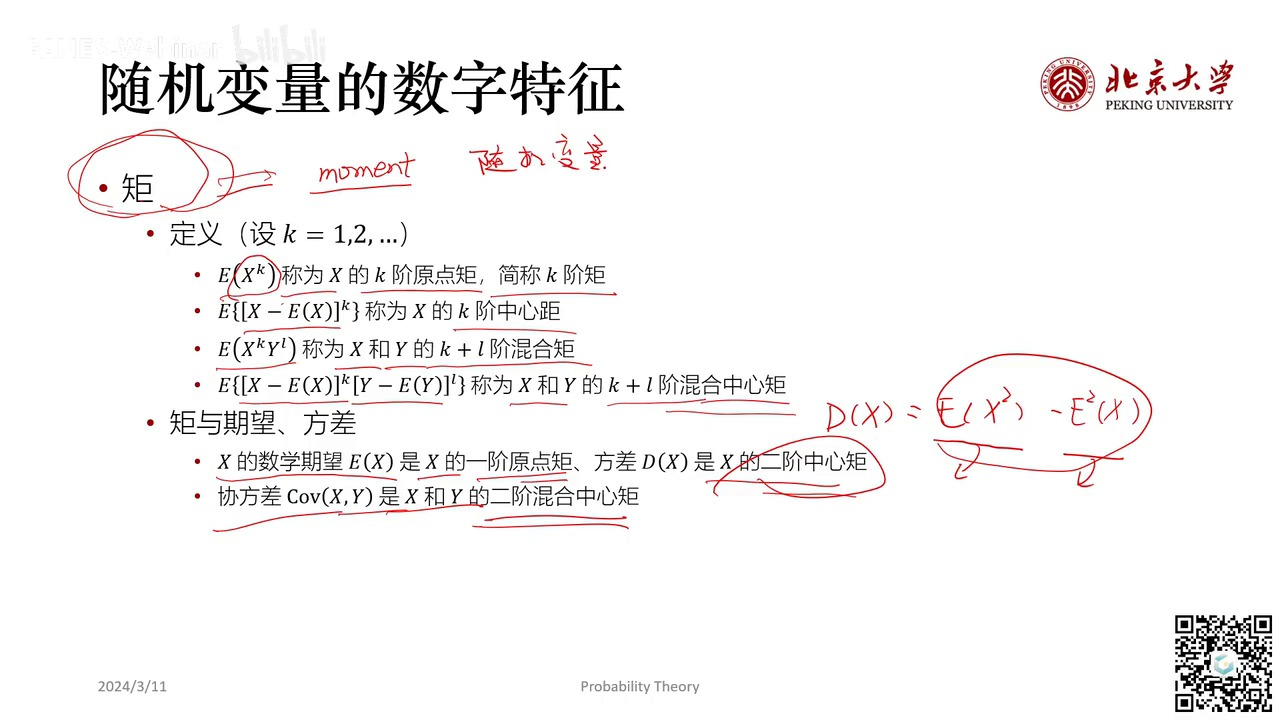
\includegraphics[width=0.92\textwidth]{figures/fig_19_moments_note.jpg}
\caption{讲者在矩的定义旁补写的关系式\vtag}
\end{figure}
\srcnote{01:00:15--01:00:30}
\end{minipage}


讲者解释，矩的英文是 moment。在概率中它是随机变量性质的反映；在统计中，我们往往只能观察样本，无法直接得到分布函数，只能通过观察各阶矩来推测分布函数大概长什么样。

\subsection{协方差矩阵}

\noindent\begin{minipage}{\textwidth}
\begin{figure}[H]
\centering
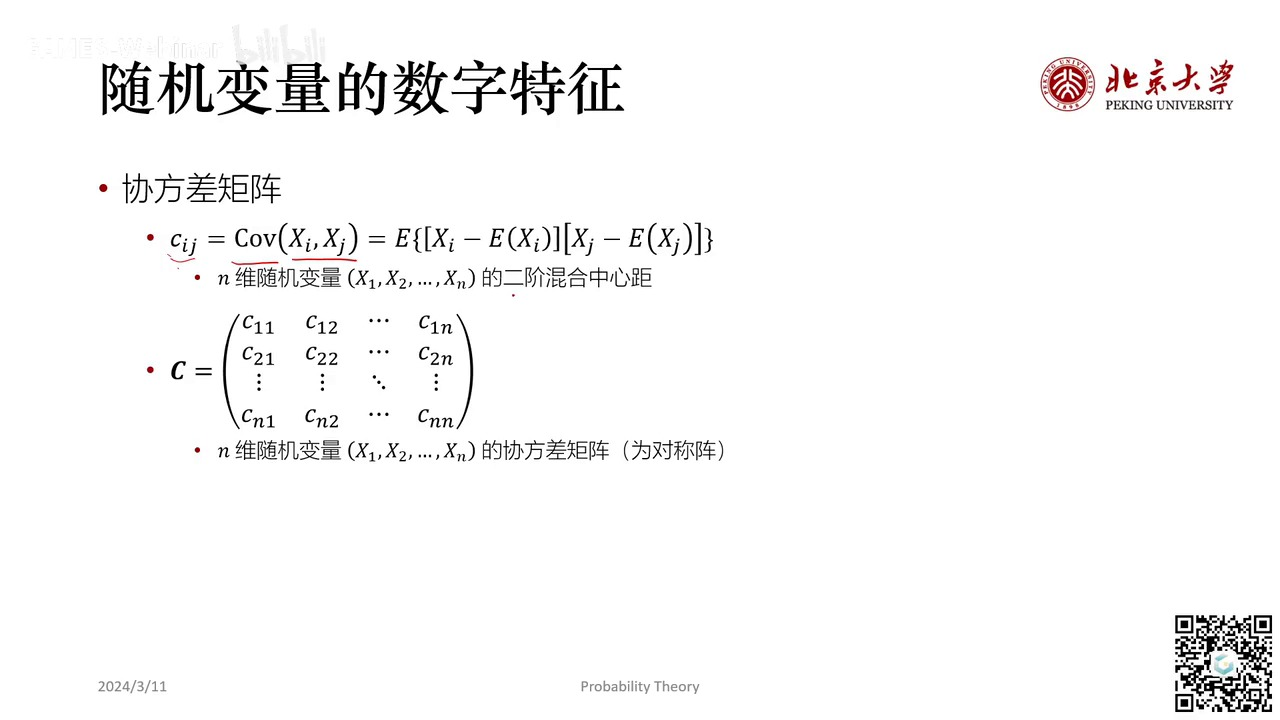
\includegraphics[width=0.92\textwidth]{figures/fig_20_covmatrix.jpg}
\caption{$n$ 维随机变量的协方差矩阵\vtag}
\end{figure}
\srcnote{01:01:30--01:01:45}
\end{minipage}


对 $n$ 维随机变量 $(X_1,X_2,\dots,X_n)$，记 $c_{ij}=\operatorname{Cov}(X_i,X_j)=E\{[X_i-E(X_i)][X_j-E(X_j)]\}$，即二阶混合中心矩，把它们排成矩阵
\begin{equation}
\mathbf{C}=\begin{pmatrix}
c_{11}&c_{12}&\cdots&c_{1n}\\
c_{21}&c_{22}&\cdots&c_{2n}\\
\vdots&\vdots&\ddots&\vdots\\
c_{n1}&c_{n2}&\cdots&c_{nn}
\end{pmatrix},
\end{equation}
称为协方差矩阵。由于协方差的对称性，它显然是对称矩阵。讲者说明了它的用处：在统计调研中得到 $n$ 个随机变量，不知道它们之间是什么关系，想考察哪个变量和哪个变量之间可能有关联，就可以计算协方差矩阵来观察。

\begin{knowledgebox}{与第五讲的联系}
讲义作者补充：第五讲的主成分分析正是对数据的协方差矩阵做特征分解（或对中心化数据做奇异值分解），特征向量给出数据变化最大的方向。协方差矩阵对称且半正定，所以特征值都非负、特征向量可以取成正交的。
\end{knowledgebox}

\section{大数定律}

\noindent\begin{minipage}{\textwidth}
\begin{figure}[H]
\centering
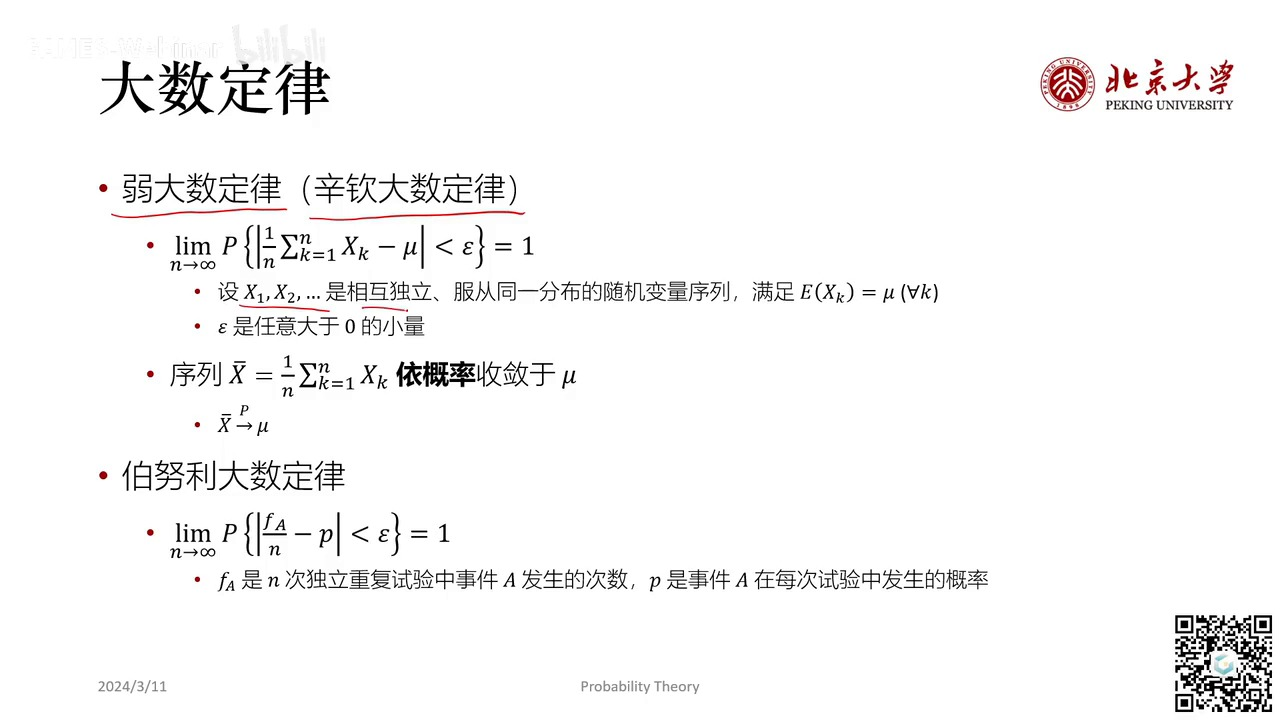
\includegraphics[width=0.92\textwidth]{figures/fig_21_lln.jpg}
\caption{弱大数定律（辛钦大数定律）与伯努利大数定律\vtag}
\end{figure}
\srcnote{01:03:15--01:03:30}
\end{minipage}


最后来看大数定律和中心极限定理。首先是弱大数定律，又叫辛钦大数定律：设 $X_1,X_2,\dots$ 是相互独立、服从同一分布的随机变量序列，且 $E(X_k)=\mu$。则对任意大于零的小量 $\varepsilon$，
\begin{equation}
\lim_{n\to\infty}P\left\{\left|\frac{1}{n}\sum_{k=1}^{n}X_k-\mu\right|<\varepsilon\right\}=1 .
\end{equation}
用更精炼的语言：记随机变量序列的平均值 $\bar X=\frac{1}{n}\sum_{k=1}^{n}X_k$，称 $\bar X$ 依概率收敛于 $\mu$，记为 $\bar X\xrightarrow{P}\mu$。

\noindent\begin{minipage}{\textwidth}
\begin{figure}[H]
\centering
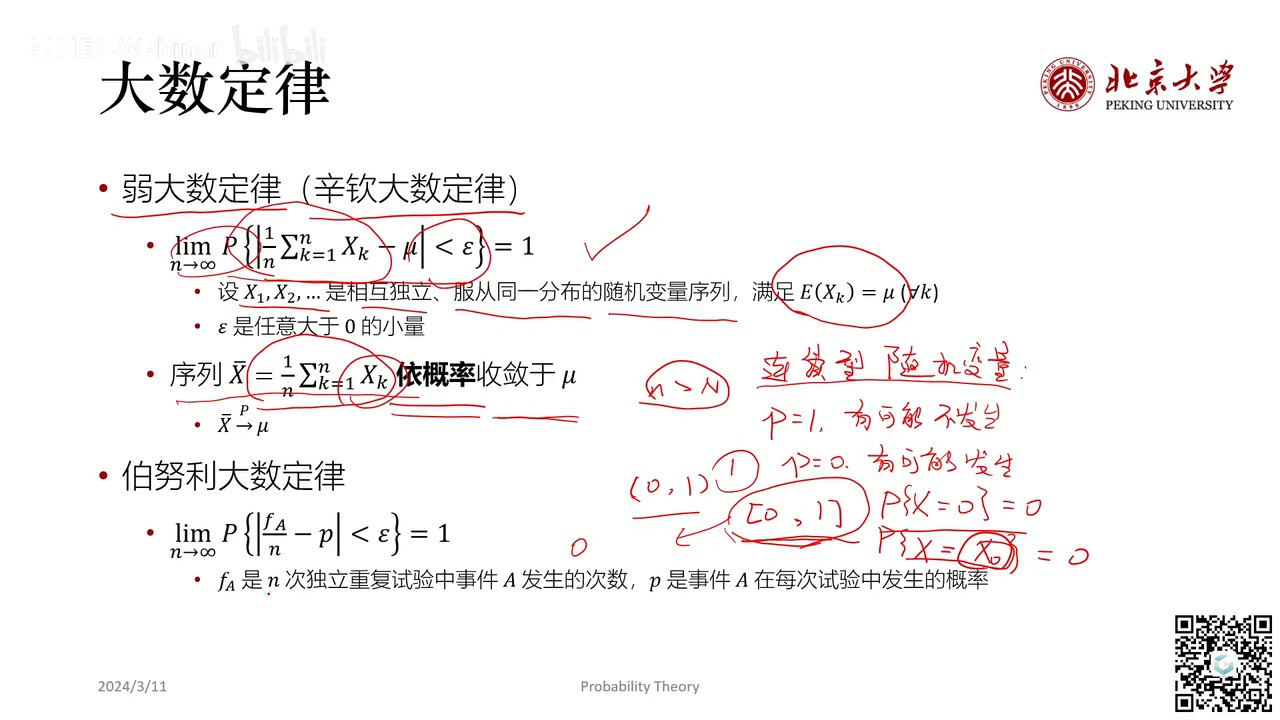
\includegraphics[width=0.92\textwidth]{figures/fig_22_lln_note.jpg}
\caption{讲者在“依概率收敛”旁的批注\vtag}
\end{figure}
\srcnote{01:07:30--01:07:45}
\end{minipage}


\begin{knowledgebox}{概率为一不等于必然发生}
讲者借此强调：对连续型随机变量来说，概率等于一的事件有可能不发生，概率为零的事件有可能发生。最简单的例子是 $[0,1]$ 上的均匀分布：实数有无穷多个，返回恰好等于某个确切值 $x_0$ 的概率是零，但做完试验后，必然得到某个确切的数，而它在试验前的概率也是零。同样，取到的随机数落在开区间 $(0,1)$ 内的概率是一，但仍有可能返回端点零。所以“依概率收敛”说的是偏离的概率趋于零，而不是保证不偏离。
\end{knowledgebox}

伯努利大数定律是它的特例：设 $f_A$ 是 $n$ 次独立重复试验中事件 $A$ 发生的次数，$p$ 是事件 $A$ 在每次试验中发生的概率，则
\begin{equation}
\lim_{n\to\infty}P\left\{\left|\frac{f_A}{n}-p\right|<\varepsilon\right\}=1 .
\end{equation}
以抛硬币为例，正面的概率是百分之五十，随着试验次数越来越大，正面出现的频率一定趋向于二分之一。这正是开头“频率趋于概率”的严格表述。

\section{中心极限定理}

\subsection{独立同分布的中心极限定理}

\noindent\begin{minipage}{\textwidth}
\begin{figure}[H]
\centering
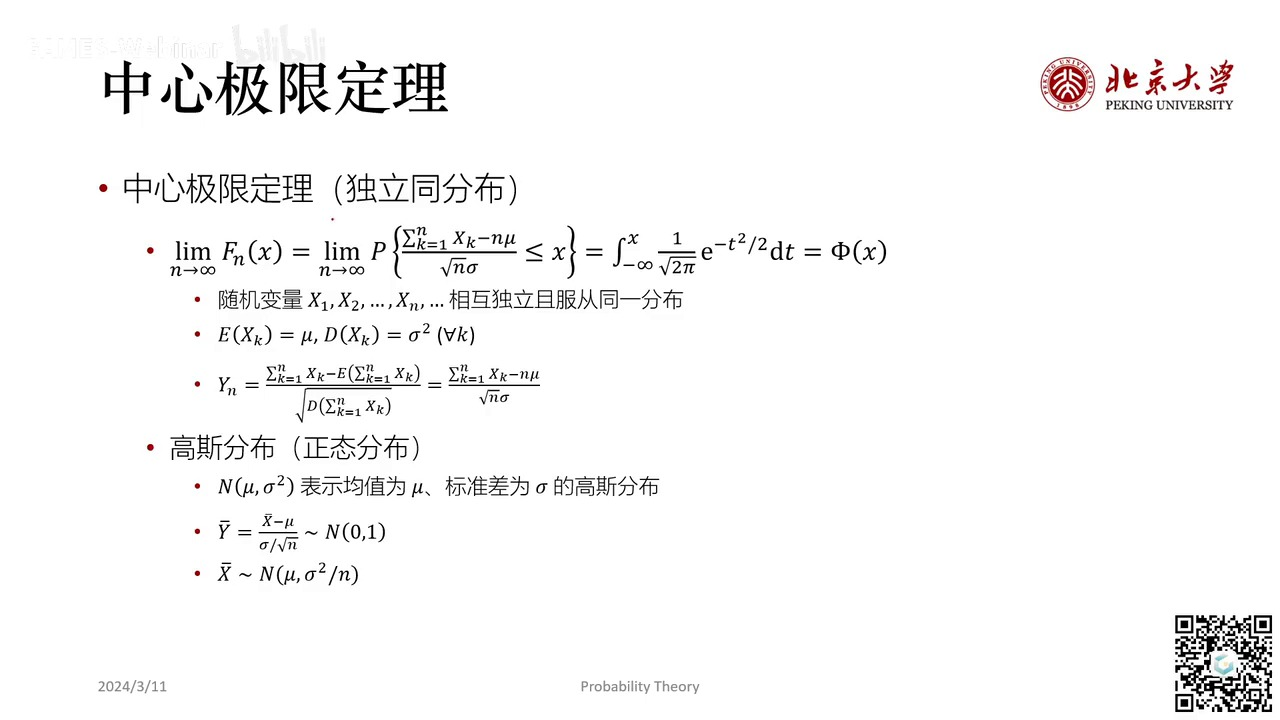
\includegraphics[width=0.92\textwidth]{figures/fig_23_clt.jpg}
\caption{独立同分布的中心极限定理与高斯分布\vtag}
\end{figure}
\srcnote{01:08:45--01:09:00}
\end{minipage}


设 $X_1,X_2,\dots,X_n,\dots$ 相互独立且服从同一分布，$E(X_k)=\mu$，$D(X_k)=\sigma^2$。定义标准化的和
\begin{equation}
Y_n=\frac{\sum_{k=1}^{n}X_k-E\left(\sum_{k=1}^{n}X_k\right)}{\sqrt{D\left(\sum_{k=1}^{n}X_k\right)}}
=\frac{\sum_{k=1}^{n}X_k-n\mu}{\sqrt{n}\,\sigma},
\end{equation}
则它的分布函数 $F_n(x)$ 满足
\begin{equation}
\lim_{n\to\infty}F_n(x)=\int_{-\infty}^{x}\frac{1}{\sqrt{2\pi}}e^{-t^2/2}\,\mathrm{d}t=\Phi(x),
\end{equation}
即标准正态分布的分布函数。

\noindent\begin{minipage}{\textwidth}
\begin{figure}[H]
\centering
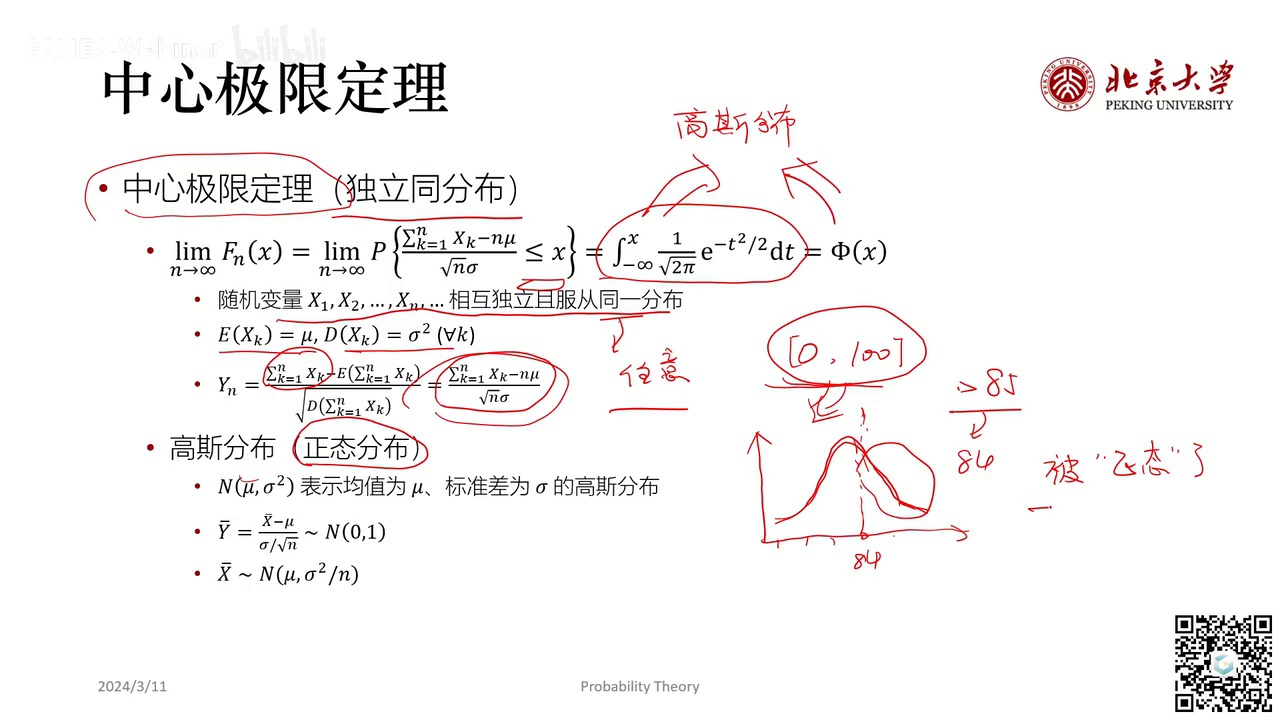
\includegraphics[width=0.92\textwidth]{figures/fig_24_clt_note.jpg}
\caption{讲者画出原分布与和的分布逐渐变成钟形曲线的示意\vtag}
\end{figure}
\srcnote{01:12:45--01:13:00}
\end{minipage}


讲者强调，这里根本没有对每个随机变量本身服从什么分布做任何假设，只要独立同分布、期望和方差存在，它们的和标准化之后就趋于高斯分布。他举例说，在一场考试中，同学们的成绩可能是零到一百上的某种分布，未必是钟形；但大量独立随机量的和或平均，就会呈现钟形。

用 $N(\mu,\sigma^2)$ 表示均值为 $\mu$、标准差为 $\sigma$ 的高斯分布（正态分布），上述结论可以简记为
\begin{equation}
\frac{\bar X-\mu}{\sigma/\sqrt{n}}\sim N(0,1)\ (\text{近似}),\qquad \bar X\sim N\!\left(\mu,\sigma^2/n\right)\ (\text{近似}).
\end{equation}

\begin{importantbox}{对蒙特卡洛方法意味着什么}
讲义作者补充：$\bar X$ 的方差是 $\sigma^2/n$，标准差是 $\sigma/\sqrt n$。在蒙特卡洛积分中，$\bar X$ 就是用 $n$ 个样本得到的估计值，所以误差按 $1/\sqrt n$ 下降：样本数增加到四倍，噪声才减半。这也是渲染中降低 $\sigma$（例如重要性采样）比单纯增加样本更划算的原因。
\end{importantbox}

\subsection{李雅普诺夫定理}

\noindent\begin{minipage}{\textwidth}
\begin{figure}[H]
\centering
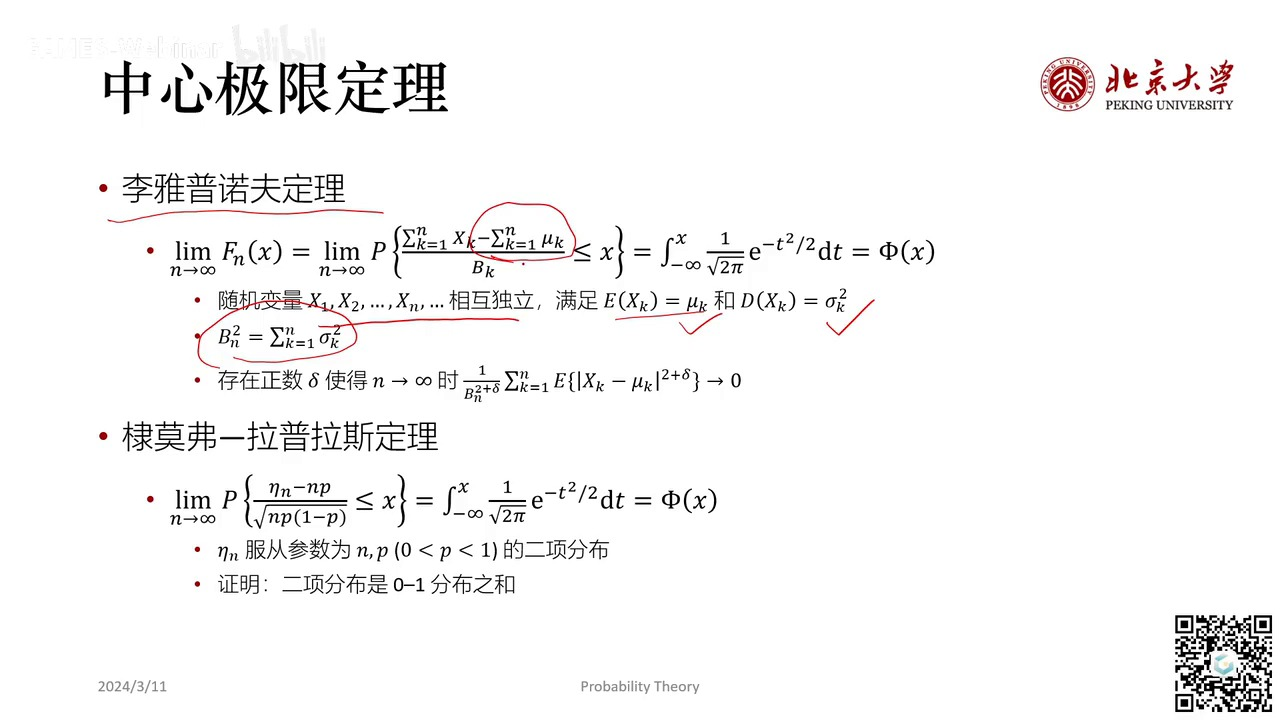
\includegraphics[width=0.92\textwidth]{figures/fig_25_lyapunov.jpg}
\caption{李雅普诺夫定理与棣莫弗—拉普拉斯定理\vtag}
\end{figure}
\srcnote{01:14:15--01:14:30}
\end{minipage}


如果随机变量不同分布呢？设 $X_1,X_2,\dots,X_n,\dots$ 相互独立，各自有期望 $E(X_k)=\mu_k$ 和方差 $D(X_k)=\sigma_k^2$。定义 $B_n^2=\sum_{k=1}^{n}\sigma_k^2$，即所有方差之和。若存在正数 $\delta$，使得当 $n\to\infty$ 时
\begin{equation}
\frac{1}{B_n^{2+\delta}}\sum_{k=1}^{n}E\left\{|X_k-\mu_k|^{2+\delta}\right\}\to 0,
\end{equation}
则
\begin{equation}
\lim_{n\to\infty}P\left\{\frac{\sum_{k=1}^{n}X_k-\sum_{k=1}^{n}\mu_k}{B_n}\le x\right\}=\Phi(x).
\end{equation}
讲者说这个定理的证明比较繁琐，大家只需要知道：把任意一些（满足一定条件的）独立随机变量加在一起，它们的和就近似服从高斯分布。

\noindent\begin{minipage}{\textwidth}
\begin{figure}[H]
\centering
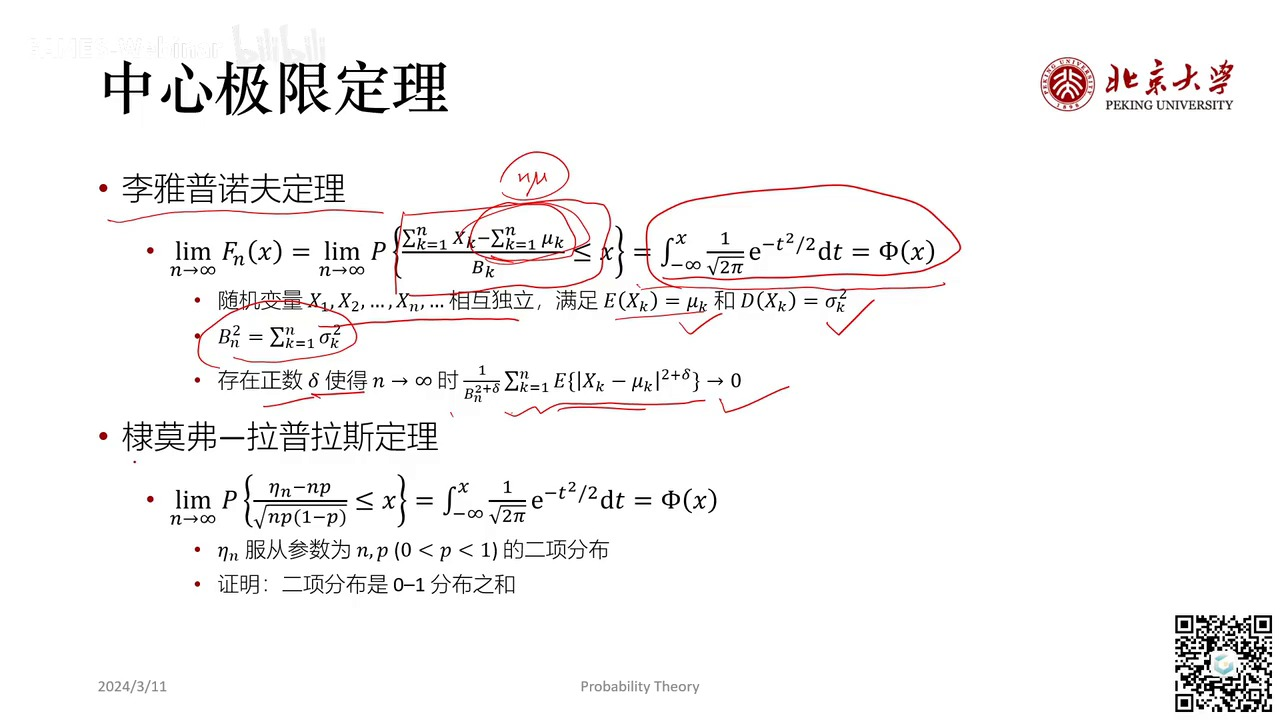
\includegraphics[width=0.92\textwidth]{figures/fig_26_lyapunov_note.jpg}
\caption{讲者对李雅普诺夫条件的批注\vtag}
\end{figure}
\srcnote{01:15:30--01:15:45}
\end{minipage}


\subsection{棣莫弗—拉普拉斯定理}

设 $\eta_n$ 服从参数为 $n,p\ (0<p<1)$ 的二项分布，则
\begin{equation}
\lim_{n\to\infty}P\left\{\frac{\eta_n-np}{\sqrt{np(1-p)}}\le x\right\}=\Phi(x).
\end{equation}

\noindent\begin{minipage}{\textwidth}
\begin{figure}[H]
\centering
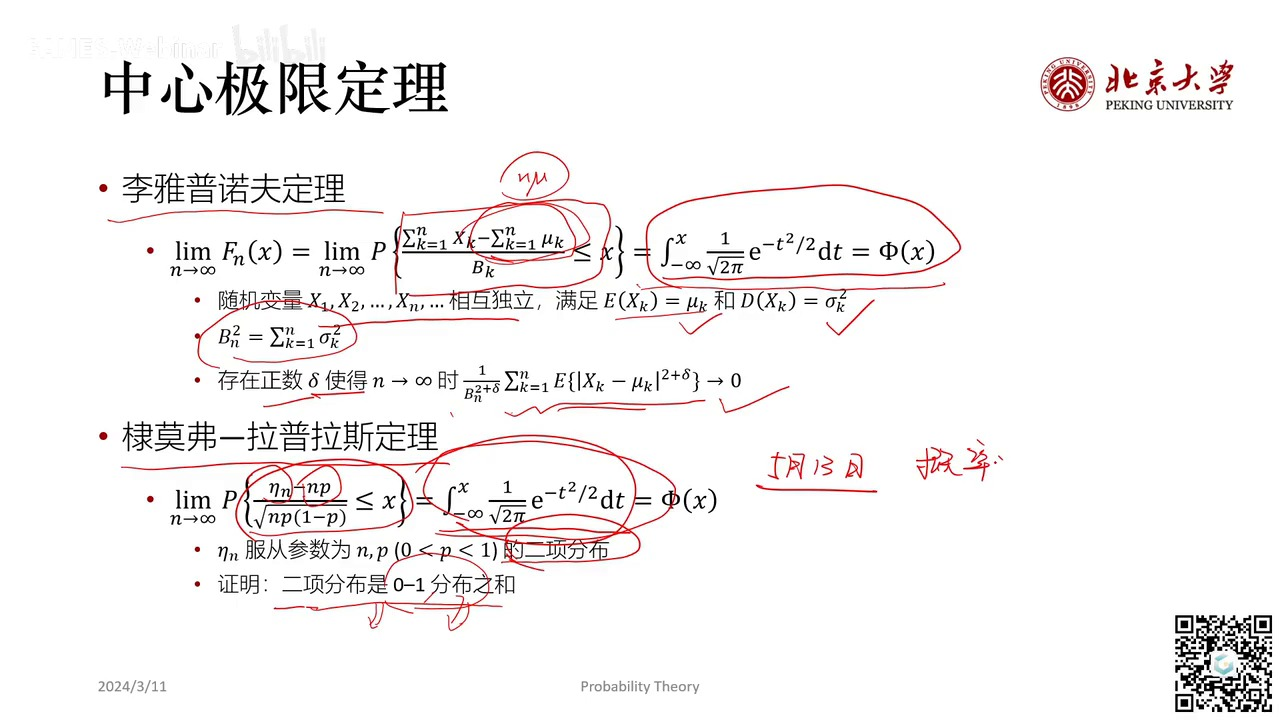
\includegraphics[width=0.92\textwidth]{figures/fig_27_demoivre.jpg}
\caption{讲者用“二项分布是 0--1 分布之和”说明棣莫弗—拉普拉斯定理\vtag}
\end{figure}
\srcnote{01:18:30--01:18:45}
\end{minipage}


证明思路是：二项分布是 $n$ 个独立 0--1 分布之和。每个 0--1 分布以 $p$ 的概率取一、以 $1-p$ 的概率取零，所以期望是 $p$，方差是 $p(1-p)$；于是二项分布的期望是 $np$，方差是 $np(1-p)$，直接套用独立同分布的中心极限定理即得。它告诉我们：二项分布的极限是高斯分布。

\begin{practicebox}{自测}
\begin{enumerate}
\item 用条件概率的定义推出乘法定理和贝叶斯公式。
\item 证明 $D(X)=E(X^2)-[E(X)]^2$，并由此求 $[0,1]$ 上均匀分布的方差（答案为 $1/12$）。
\item 写出指数分布的无记忆性，并说明它为什么与“已经等了多久”无关。
\item 解释为什么 $\operatorname{Cov}(X,Y)=0$ 不能推出 $X,Y$ 独立，并给一个例子。
\item 若一个蒙特卡洛估计用 $100$ 个样本时标准差为 $0.1$，要把标准差降到 $0.01$ 大约需要多少样本？（答案：$10000$。）
\end{enumerate}
\end{practicebox}

\section{小结}

讲者对本讲做了简单总结：从频率出发定义了概率，介绍了古典概型和条件概率；引入随机变量，讨论了常见的离散与连续分布；用期望、方差、协方差和矩来刻画分布；最后介绍了大数定律和中心极限定理，它们说明大量重复的平均会稳定在期望附近，而且偏差近似服从高斯分布。

讲者在结尾祝大家假期愉快，并说明下周一是假期，休息一次，下下周一再继续。概率论的第二部分将在五月十三日讲完，之后发布概率论部分的作业。

\begin{knowledgebox}{下一讲预告}
本讲只回顾了概率论的基础。下一讲（概率论二）会进入与图形学联系更紧密的内容，例如随机数采样与蒙特卡洛积分；本讲的期望、方差和中心极限定理是理解这些方法的前提。
\end{knowledgebox}

\end{document}
